\documentclass[a4paper]{article}
% The web build uses the project's small, LaTeXML-compatible style layer.
% The original kod.sty is retained beside this file for the standalone PDF,
% but its tcolorbox/expl3 stack is not needed by the manuscript itself.
\usepackage{mmp}
\usepackage{float}

\newcommand{\ord}{\operatorname{ord}}

%%%%%%%%%%%%%%%%%%%%%%%%%%%%%%%%%%%%%%%%%%%%%%%%%%

\title{\vspace*{10mm}\bf The Method of Moving Points\\
-\\
For contestants} % Cím vagy téma ide

\author{Molnár-Szabó Vilmos\\ \href{mailto:vilmosmolnarszabo@gmail.com}{vilmosmolnarszabo@gmail.com}} % Szerző neve és email címe ide

\date{} % MARADJON ÜRESEN
%%%%%%%%%%%%%%%%%%%%%%%%%%%%%%%%%%%%%%%%%%%%%%%%%%

% Új parancs létrehozása: \newcommand{\parancs}{mit írjon ki}

% A híres számhalmazok parancsai az adott kisbetű kétszer, például a természetes számok halmaza \nn

%%%%%%% START %%%%%%%%%%

\begin{document}

\maketitle

\tableofcontents

%%%%%%%%%%%%%%%%%%%%%%%%%%%%%%%%%%%%%%%%%%%%%%%%%%
\section{Introduction}

This document is about the Method of Moving Points - a powerful geometry problem solving method. With the help of it even the hardest problems on the IMO shortlist are solvable. In my experience the most effective is to combine synthetic, and the MMP, that means starting with synthetic techniques, simplifying the figure or the statement so that it can be easily solved with the MMP.

The document consists of the basic version of the method\cite{animation}\cite{mmp}, and the further extensions made by me. You can also find exercises, where you can practice the most common situations appearing in problem solving. You need paper and pen at these parts.

The necessary knowledge are
\begin{itemize}
    \item projective plane
    \item homogeneous coordinates
    \item projective transformation of the plane
    \item inversion
    \item pole-polar
\end{itemize}

Furthermore, there are proofs that use basic linear algebra, but it's not necessary to understand each proof, so go ahead if you're not familiar with linear algebra.

I made a video about the basics of the method, where I also explain the projective plane and the homogeneous coordinates:

\url{https://youtu.be/nJne30M9ijo?si=b24iNYWvMXim07Z3}

I'm still doing research in MMP, and if you have any idea, or question about it, please write me an email.

I'll update this document regularly, so check out the description of the video for updates.

Have fun exploring this beautiful topic!

\section{Moving points and lines}

\subsection{Moving points}

A polynomial moving point is a time dependent point on the projective plane. We denote the points of the projective plane by homogeneous coordinates.

\begin{definition}
\hfill\break
A polynomial moving point is defined by three polynomials in the following way:

$$H(t)=(p(t):q(t):r(t))$$

To avoid getting $(0:0:0)$, $p$, $q$ and $r$ must have no common root.

The degree of $H$ is defined to be $\max(\deg p, \deg q, \deg r)$.




\end{definition}
    
\begin{remark}
    At $t=\infty$ we define $H$ to be the limes of itself, as $t\rightarrow \infty$.
\end{remark}
To give you a picture:



\begin{lemma}
\hfill\break
    Degree 0 points are fixed.

    A degree 1 point always moves on a line, and it passes through each point exactly once. (with multiplicity)

    A degree 2 point always moves on a conic, passing through each point once, or on a line, in which case it passes through every point twice.
    (with multiplicity)
\end{lemma}

\begin{remark}[Multiplicity]
    Certain events can happen with multiplicity, for example the coincidence of two points. This means that at a time, they can coincide 'with multiplicity $n$', so it counts as $n$ coincidences instead of one. The concept is the same as the multiplicity of the root of a polynomial.%The multiplicity of the coincidence of two points is the order of zero of their distance. This means that if the distance is not just zero, but its derivative is also zero, then the multiplicity is at least 2.
\end{remark}


\begin{remark}[We are over $\cc$]
    We also allow time to be a complex number, and a moving point to have complex coordinates. You don't have to imagine 4d space, just stay with the plane and accept that the coordinates can be complex numbers also. This way everything becomes much more well-behaving, for example every line and circle has 2 intersection points (with multiplicity). This is just like every degree 2 polynomial has 2 roots over complex numbers with multiplicity.
\end{remark}

\subsection{Moving lines}

We can define polynomial moving lines the same way as we defined points:

\begin{definition}
A polynomial moving line is defined by three polynomials in the following way:

$$L(t)=(p(t):q(t):r(t))$$

To avoid getting $(0:0:0)$, $p$, $q$ and $r$ must have no common root.

The degree of $H$ is defined to be $\max(\deg p, \deg q, \deg r)$.
\end{definition}

\begin{remark}
    At $t=\infty$ we define $L$ to be the limes of itself, as $t\rightarrow \infty$.
\end{remark}

And to help you imagine moving lines:

\begin{lemma}
\hfill\break
    Degree 0 lines are fixed.

    A degree 1 line always rotates around a fixed point, and takes all its positions once. (with mul.)

    A degree 2 line is either always tangent to a conic, and takes all its positions once, or it rotates around a fixed point, and takes all its positions twice. (with mul.)
\end{lemma}


\section{Degree of statements}



Most of the statements occurring in geometry problems are true a certain number of times as time varies (with multiplicity), or they are always true. This number is called the degree of the statement. If we can show that the statement happens degree+1 times, it implies that the statement is always true!

\subsection{P lies on l}

\begin{theorem}\label{point-line}
    Let $P$ be a polynomial moving point, and let $l$ be a polynomial moving line. Then the degree of the statement "$P$ lies on $l$" is exactly $\deg P+ \deg l$. 
\end{theorem}
\begin{proof}
    $\deg l=a$ and $\deg P=b$.

    The statement "P lies on l" is equivalent to $l_1\cdot p_1+l_2\cdot p_2+l_3\cdot p_3=0$. This a degree $a+b$ polynomial of time.
    
    By the fundamental theorem of algebra, the polynomial $l_1\cdot p_1+l_2\cdot p_2+l_3\cdot p_3$ has exactly $a+b$ zeros with multiplicity, or it is constant zero, so $p$ is on $l$ exactly $a+b$ times or always.
\end{proof}
\subsection{A, B, C are collinear}
\begin{theorem}\label{deg3p}
    Let $A$, $B$, $C$ be three polynomial moving points. Then the degree of the statement "$A$, $B$, $C$ are collinear" is exactly $\deg A+ \deg B+ \deg C$.
\end{theorem}
\begin{remark}
    When two out of the three points coincide, it counts as being collinear. For further details about multiplicity, see chapter Multiplicities~\ref{mul}.
\end{remark}
\begin{proof}

(for those who know basic linear algebra)
\[
A = (a_1, a_2, a_3) \quad 
B = (b_1, b_2, b_3) \quad 
C = (c_1, c_2, c_3)
\]
where $a_i, b_i, c_i$ are degree $\deg A, \deg B, \deg C$ polynomials of time respectively.

    The statement is equivalent to
\[
\det \begin{pmatrix}
a_1 & a_2 & a_3 \\
b_1 & b_2 & b_3 \\
c_1 & c_2 & c_3
\end{pmatrix} = 0
\]

When the determinant is expanded, it is an $a+b+c$ degree polynomial of time, so it has exactly $a+b+c$ roots with multiplicity over $\cc$.
\end{proof}

\subsection{e, f, g are concurrent}

\begin{theorem}
    Let $e$, $f$, $g$ be three polynomial moving lines. Then the degree of the statement "$e$, $f$, $g$ are concurrent" is exactly $\deg e+ \deg f+ \deg g$.
\end{theorem}
\begin{remark}
    When two out of the three lines coincide, it counts as being concurrent. For further details about multiplicity, see chapter Multiplicities~\ref{mul}.
\end{remark}
\begin{proof}
    Take the previous proof, and swap the role of points and lines, and change collinearity to concurrency.
\end{proof}

\subsection{A=B on a fixed line}

\begin{theorem}\label{degab}
    Let $A$ and $B$ be two polynomial moving points on a fixed line. Then the degree of the statement "$A$=$B$" is exactly $\deg A+ \deg B$.
\end{theorem}
\begin{proof}
    Take an arbitrary fixed point $F$ that isn't on the fixed line. Then "$A=B$" is equivalent to "$F, A, B$ are collinear", and this has degree $\deg F+\deg A+\deg B=\deg A+\deg B$, because $\deg F=0$.
\end{proof}

\subsection{A=B on a fixed conic}

\begin{theorem}
    Let $A$ and $B$ be two polynomial moving points on a fixed conic. Then the degree of the statement "$A$=$B$" is $\frac{\deg A+ \deg B}{2}$.
\end{theorem}
\begin{proof}
    See section Mászó-theorem~\ref{maszo}
\end{proof}

\begin{remark}
    Ideal points, and the ideal line are to be treated equally to normal points and lines, so for example if three moving points $A$, $B$, and $C$ become ideal points at the same time, the statement "$A, B, C$ are collinear" is true, since they are on the ideal line.
    Whenever a you're not sure if something counts or not, just because some ideal point/line is involved, it counts.
\end{remark}
\section{Constructing new objects}

Suppose we know the degree of some polynomial moving points or lines, and we construct a further point or line from them. We are interested in the degree of the new object. In this section we'll go through some of the basic construction steps, and the formulas for calculating the degree of the new object.

\begin{remark}
    When constructing the new object, it can happen that at a time $t_0$ the construction becomes degenerate, or it is not defined. Then we define the new object as the limes of itself as $t\rightarrow t_0$.
    For example if two points are moving on a circle, and they coincide at $t_0$, then the line through them will be the tangent to the circle at that point.
\end{remark}

\subsection{Line through two points}

The next theorem is the most used one in problem solving, so learn it well.

\begin{theorem}[Zack's lemma]\label{l-pp}
    Let $A$ and $B$ be two polynomial moving points. Then the line $AB$ is polynomial and its degree is

$$\deg (AB)= \deg (A) + \deg (B) - \# (A=B)$$

where $\# (A=B)$ denotes the number of times when $A=B$ (with multiplicity). This includes complex times and $t=\infty$ also.
\end{theorem}
\begin{proof}
    Take an arbitrary fixed point $F$ neither on the locus of $A$ or the locus of $B$.

    Since $F$ has degree 0, the degree of the statement "$F$ is on line $AB$" is $\deg AB$. The statement "$A, B, F$ are collinear" is equivalent to ("$F$ is on line $AB$" \it{or} \rm "$A=B$") Therefore if we count both of them as time varies, we get
    $$\deg (A) + \deg (B)= \deg (AB) + \# (A=B)$$
    from which the statement follows.
\end{proof}

\begin{remark}
    A common theme in the construction step formulas is the $-\#("\text{event}")$ part. Here the "event" is always when the constructed object is not unique. For example in Zack's lemma, the line through two points is not unique exactly when the two points coincide, that is $A=B$.
\end{remark}

\subsection{Point of intersection of two lines}
The dual statement of the previous theorem is also referred to as Zack's lemma:

\begin{theorem}\label{p-ll}
    Let $e$ and $f$ be two polynomial moving lines. Then the intersection point $e\cap f$ is polynomial and its degree is

$$\deg (e\cap f)= \deg (e) + \deg (f) - \# (e=f)$$

where $\# (e=f)$ denotes the number of times when $e=f$ (with multiplicity). This includes complex times and $t=\infty$ also.
\end{theorem}

\begin{proof}
    The proof is the same as of the previous theorem, but the role of points and lines are swapped.
\end{proof}
\subsection{Projective transformation}
Every projective transformation preserves degrees:
\begin{theorem} 
    Let $\mathcal{A}$ be a projective transformation of the plane, $P$ a polynomial moving point, and $l$ a polynomial moving line. Then $\deg P=\deg \mathcal{A}(P)$ and $\deg l=\deg \mathcal{A}(l)$
\end{theorem}

\begin{proof}
    A projective transformation can be written as
    \[
(x : y : z) \mapsto 
(a_1 x + b_1 y + c_1 z : 
 a_2 x + b_2 y + c_2 z : 
 a_3 x + b_3 y + c_3 z)
\]


for some $a_i, b_i, c_i \in \cc$, where both sides denote points, or both sides denote lines.

If $x,y,z$ are degree $n$ polynomials of time, then the result will also be degree $n$.

\end{proof}
\begin{corollary}
    Every isometry, homothety, affine and projective transformation preserves degrees, including rotation, mirroring, scaling and translation. (Where does these transformations take an ideal point? Think it through.)
\end{corollary}


\subsection{Pole-polar}
\begin{theorem}\label{polepolar deg}
    Let $\mathcal{C}$ be any nondegenerate conic, and let $P$ and $l$ be a point and line with pole-polar relation with respect to $\mathcal{C}$. Then $\deg (P)=\deg (l)$.
\end{theorem}

\begin{proof}
    A pole polar transformation can be written as
    \[
(x : y : z) \mapsto 
(a_1 x + b_1 y + c_1 z : 
 a_2 x + b_2 y + c_2 z : 
 a_3 x + b_3 y + c_3 z)
\]


for some $a_i, b_i, c_i \in \cc$, where the left hand side denotes a point, while the right hand side denotes a line.

If $x,y,z$ are degree $n$ polynomials of time, then the result will also be degree $n$.
\end{proof}


\subsection{Midpoint}
\begin{theorem}
    Let $A$ and $B$ be two points with midpoint $M$. Then
    $$\deg M=\deg A+ \deg B - \#(A \text{ and } B \text{ are both ideal points})$$
\end{theorem}
\begin{remark}
    The method of calculating the multiplicity of $\#(A \text{ and } B \text{ are both ideal points})$ is not yet known, but taking this number without multiplicity gives an upper bound on $\deg M$ which is sufficient to prove your problem in most cases.
\end{remark}
\begin{remark}
    This formula is also true, when $M$ has any fixed division ratio with respect to $A$ and $B$. Moreover the formula works if $M$ is moving such that triangle $ABM$ is always similar to a fixed triangle. In other words if angles $\angle ABM$ and $\angle BAM$ are fixed.
\end{remark}


\section{Proving geometry problems}



\begin{lemma}
    For every line $l$, there exists a degree 1 point $P$, such that the locus of $P$ is $l$.

    For every conic $\mathcal{C}$, there exists a degree 2 point $P$, such that the locus of $P$ is  $\mathcal{C}$.
\end{lemma}

We finally came to the point where we have the necessary tools to use the method.

A geometry problem usually takes the following format: There are some initial objects, from which we construct further objects, and then we have to prove a statement about some of these objects.

We first take any configuration of the initial objects, and we want to prove the statement for this configuration. We fix some of the initial objects. Then we 'animate' one of the initial objects, this will be the 'initial moving point'. We choose a locus (line or conic) to the initial point, and animate it to move like a degree 1 polynomial point if the locus is a line, or a degree 2 polynomial point if the locus is a conic.

There is a sequence of objects in which they are defined, each object is constructed using the previous ones, just like as they are defined in the problem. So the rest of the objects are moving along with the initial moving point.

Then we can calculate the degree of the constructed objects one by one using the construction step formulas.

We then calculate the degree of the statement from the degrees of the points and lines involved in it.

Finally we find degree+1 special cases, where the statement is true. We can choose simpler or degenerate configurations for special cases. This proves that at every position of the initial point the statement is true, specifically at the place from where we 'started' the animation, which was a general configuration.

Here is an example problem with solution.

\begin{exercise} [Gergonne-point]
    In triangle $ABC$ the tangency points of the incircle are $D$, $E$ and $F$ on sides $BC$, $CA$ and $AB$ respectively. Prove that $AD$, $BE$ and $CF$ are concurrent.
\end{exercise}
\begin{proof}
    \begin{figure}[H]
    \centering
    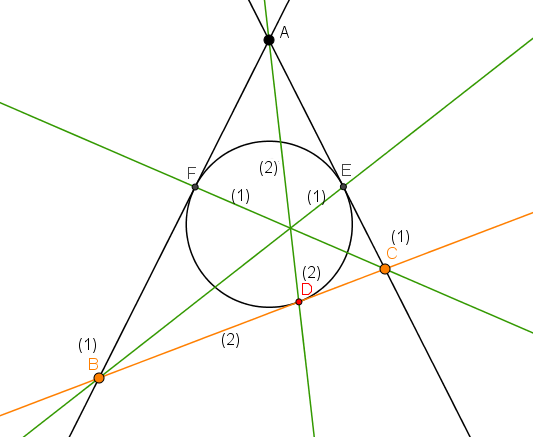
\includegraphics[width=0.7\textwidth]{kepek/kep0.png}
    \caption{The incircle animation. Drag the point and inspect the degree calculation.}
    \label{fig:gergonne}
    \end{figure}

    We use the incircle-animation, which comes up very often in problem solving, and is very useful.

    We start with a general configuration of triangle $ABC$.
    
    Let's fix $A$, $E$, $F$ and the incircle, and start animating point $D$ with degree 2 on the incircle.

    Now side $BC$, points $B$ and $C$ and lines $AD$, $BE$ and $CF$ are constructed in this order, so they are determined by $D$, meaning that they move along with $D$. We'll calculate their degrees one by one.
    
    Since side $BC$ is the polar of $D$ with respect to the incircle, $BC$ has the same degree as $D$, which is 2.

    $B$ is the intersection of the fixed side $AB$, and the degree 2 side $BC$. We can use Zack's lemma~\ref{p-ll} to calculate the degree of $B$, that is

    $$\deg B= \deg AB + \deg BC - \# (AB=BC)=0+2-1=1$$

    $AB$ coincides with $BC$ exactly once, when $D=F$, that's why we can reduce the degree by 1.

    Similarly $C$ also has degree 1.

    To calculate the degree of $EB$, we use Zack's lemma~\ref{l-pp}. That is
    $$\deg EB= \deg B + \deg E - \# (B=E)=1+0-0=1$$
    $B$ and $E$ never coincide.

    Similarly $FC$ also has degree 1.
    
    $AD$ has degree $0+2-0=2$.

    The statement "$BE$, $FC$, $AD$ are concurrent" has degree $\deg BE+\deg FC+\deg AD=1+1+2=4$.

    Then it is sufficient to find 4+1=5 special cases where the statement is true.

    \begin{enumerate}
        \item $AB=AC$
        
        Now $ABC$ is isosceles, and the statement is true for every isosceles triangle by symmetry.

        \item $BA=BC$

        Another isosceles case.
        \item $CA=CB$
        
        And another.
        \item $D=E$

        This is a degenerate case. $C=E=D$, because of the degeneration. Therefore $AD$, $BE$ and $CF$ all go through this point, so they are concurrent.

        \item $D=F$

        The symmetric pair of the previous case.
    \end{enumerate}
    Now we proved that the statement is true for every position of $D$. Therefore it is true for the original position, which was a general case, so the statement is true for every triangle $ABC$.
\end{proof}

\begin{remark}
    In the 4th case when $D=E$, $BC$ and $AC$ coincide. Then their intersection $C$ is not unique. Let's say this happened at time $t_0$. In this case we always define the position of the moving point $C$ at $t_0$ to be $\lim_{t\to t_0}C(t)$. This way the moving point $C(t)$ is continuous.
\end{remark}

\begin{remark}
    There is a quite widespread information, that we must not use the special case where we reduced degree previously. This is NOT true, in fact you CAN use any special case you want. The reason is that all the theorems state "if you find n+1 cases, you proved the statement", they don't mention any exceptions.

    However, there's a reason why people feel unsure about using a special case where we reduced degree previously. To make this clear, note that in every construction step formula, we can reduce the degree with the $-\#("\text{event}")$ part, and the event is exactly when the construction step is not defined uniquely. For example the degree of the intersection point of two lines can be reduced exactly when the two lines coincide, and thus their intersection point is not unique.

    Therefore if we reduce the degree of any object $X$ at a time $t_0$, then we are not able to tell the position of $X$ at $t_0$, unless we calculate $\lim_{t\to t_0}X(t)$. And to check the special case at $t_0$ at the end of the proof, we have to tell the position of $X$, so we can check the statement about $X$.

    In our example problem, we used the special case again when $D=E$, but to do that, we had to work a little extra: we had to tell the limit of $C$ at this moment. And of course, since $BC$ and $AC$ are both tangent to the incircle, the limit of their intersection will be the tangency point of $AC$ at $t_0$. To see this, just try to imagine the scene in your head, as $t\to t_0$. And then we used this information to determine whether the statement is true or not.

So as a conclusion, if you reduce a degree, you can use it again as a special case, but inevitably you have to calculate the limit of that object.
\end{remark}


\section{Locus of a moving point}


\begin{theorem} [Locus-theorem]\label{locus}
    Let $H$ be a degree $n$ polynomial moving point. Then the locus of $H$ is a degree $k$ irreducible algebraic curve, where $k\mid n$. $H$ passes through every smooth point of the curve $\frac{n}{k}$ times (with  mul.). $H$ passes through any order $d$ singularity $\frac{n}{k}\cdot d$ times (with mul.)
\end{theorem}

\begin{remark}
    A degree $k$ algebraic curve is the set of solutions of $p(x,y)=0$, where $p$ is a degree $k$ two-variable polynomial. For example degree 1 algebraic curves are lines, and degree 2 algebraic curves are conics.
    
    Intuitively a singularity of an algebraic curve is a point, where the curve either have self-intersection, or a point, where it 'breaks'. The order of a singularity is intuitively the number of 'branches' at the self-intersection.
    There are only finitely many singularities on a curve.
    Lines and conics don't have any singularities.

    A smooth point is a point that is not singular.
\end{remark}
\begin{example}
    A degree $n$ moving point on a fixed line goes through each point of the line $n$ times (with mul.).
\end{example}

\section{Mászó-theorem}\label{maszo}

While solving a geometry problem, calculating the degree of a line through two points takes a lot of time, because we have to  check all the coincidences of the two points. However when both points move on the same conic, Mászó-theorem gives an explicit degree of the line through them. And luckily that degree is quite low!

\begin{lemma}
    The degree of a moving point on a fixed conic is always even.
\end{lemma}

\begin{proof}
    The Locus-theorem~\ref{locus} states that if a degree $n$ point moves on a degree $k$ algebraic curve, then $k\mid n$. Here $k=2$, so $2\mid n$.
\end{proof}

\subsection{Mászó-theorem}

\begin{theorem}[Mászó-theorem]
Two polynomial points $A$ and $B$ move on the same conic. Then
$$\deg AB = \frac{\deg A+\deg B}{2}$$
    
\end{theorem}

\begin{proof}
    Let $F$ be a degree 0 fixed point on the conic.
    The event "$F$ is on line $AB$" has degree $\deg AB$, and it is equivalent to ("$A=F$" or "$B=F$"), which happen $\frac{\deg A}{2}$ and $\frac{\deg B}{2}$ times respectively by the Locus theorem. Combining these we get 
    $$\deg AB = \frac{\deg A+\deg B}{2}$$
    
\end{proof}

\subsection{Inverse Mászó-theorem}\label{invmaszo}

When we calculate the degree of the second intersection point of a circle and a line, such that the first intersection point is already given, we use the inverse Mászó-theorem.

\begin{theorem} [Inverse of Mászó-theorem]

    Let $\mathcal{C}$ be a fixed conic, $A$ is a polynomial moving point on it, and $l$ is a polynomial line always going through $A$. The second intersection of $\mathcal{C}$ and $l$ is $B$. Then $B$ is polynomial, and its degree satisfies

    $$\deg l = \frac{\deg A+\deg B}{2}$$
    
\end{theorem}
\begin{proof}

    With a projective transformation we can send any conic into a circle, so we can suppose $\mathcal{C}$ is a circle with center $O$. $l$ has a polynomial ideal point (intersection with the ideal line, which is fixed). A 90° rotation sends this ideal point into the perpendicular direction's ideal point, so connecting this with $O$ gives us a polynomial line, which is the perpendicular bisector of $A$ and $B$. A polynomial point's reflection about a polynomial line is also polynomial, and therefore $B$ is polynomial.
    
    We can now use Mászó-theorem to conclude that indeed $$\deg l = \frac{\deg A+\deg B}{2}$$
\end{proof}

The following theorem was already stated without proof, now Mászó-theorem gives us a nice proof.
\begin{theorem}
    Let $A$ and $B$ be two polynomial moving points on a fixed conic. Then the degree of the statement "$A$=$B$" is $\frac{\deg A+ \deg B}{2}$.
\end{theorem}
\begin{proof}
    Mászó-theorem:
    $\deg AB=\frac{\deg A+\deg B}{2}$
    
    Line through two point formula:
    $\deg AB=\deg A+\deg B-\#(A=B)$
    
    $\implies \#(A=B)=\frac{\deg A+\deg B}{2}$
\end{proof}



\section{Common construction steps}

In this section we'll go through some common construction steps occurring in problems, which are really important. You have to calculate the degrees yourself, so prepare a paper and a pen. At the end of the section, you'll find the solutions.

\subsection{Projection from line to line}
\label{exc_linetoline}
\begin{figure}[H]
    %\centering
    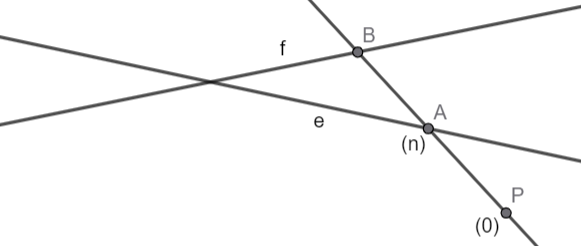
\includegraphics[width=0.6\textwidth]{kepek/kep1.png}
\end{figure}

Animation: $e$ and $f$ are fixed, $P$ is fixed, $A$ moves on $e$ with degree $n$.

Calculate the degrees of the following objects one by one in this order:
\begin{itemize}
    \item $PA$
    \item $B$
\end{itemize}

Zack's lemma ~\ref{l-pp} for line $AB$ states
$$\deg (AB)= \deg (A) + \deg (B) - \# (A=B)$$
Check that it is indeed true in this case.

Solutions: ~\ref{sol_linetoline}

\subsection{Projection between line and conic}
\label{exc_linetoconic}
\begin{figure}[H]
    %\centering
    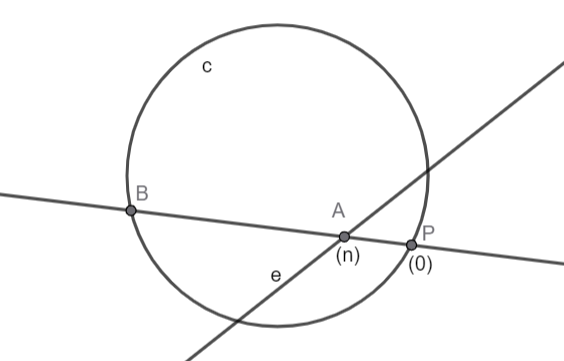
\includegraphics[width=0.6\textwidth]{kepek/kep2.png}
\end{figure}

Animation: $e$, $c$ and $P$ are fixed, $A$ moves on $e$ with degree $n$.

Calculate the degrees of the following objects one by one in this order:
\begin{itemize}
    \item $PA$
    \item $B\quad$ hint: use inverse Mászó-theorem ~\ref{invmaszo}
\end{itemize}

Solutions: ~\ref{sol_linetoconic}

\subsection{Projection from conic to itself}
\label{exc_conictoconic}

\begin{figure}[H]
    %\centering
    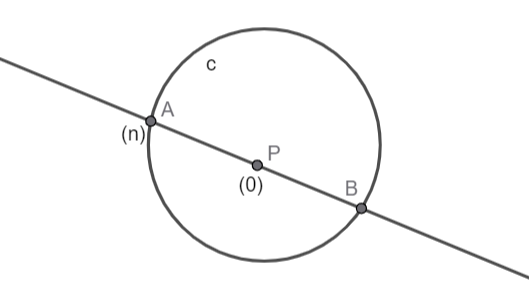
\includegraphics[width=0.6\textwidth]{kepek/kep3.png}
\end{figure}

Animation: $c$ and $P$ are fixed, $A$ moves on $c$ with degree $n$.

Calculate the degrees of the following objects one by one in this order:
\begin{itemize}
    \item $PA$
    \item $B$
\end{itemize}

Solutions: ~\ref{sol_conictoconic}

\subsection{Perpendicular projection}
\label{exc_perpproj}

\begin{figure}[H]
    %\centering
    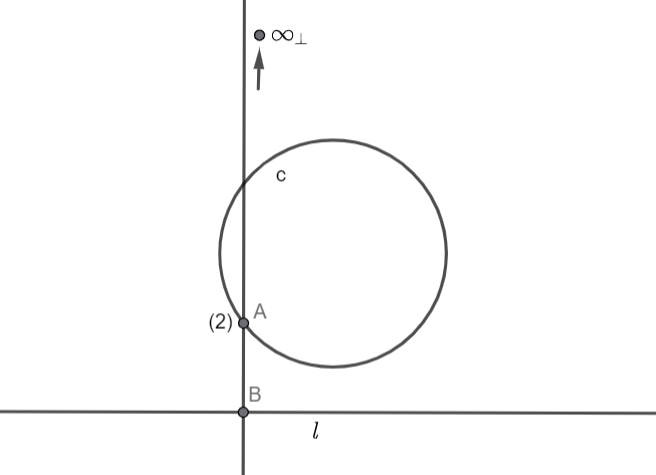
\includegraphics[width=0.6\textwidth]{kepek/kep4.png}
\end{figure}

Animation: $c$ and $l$ are fixed, $A$ moves on $c$ with degree 2.

Calculate the degrees of the following objects one by one in this order:
\begin{itemize}
    \item $\infty_{\perp}$
    \item $A\infty_{\perp}$
    \item $B$
\end{itemize}

Solutions: ~\ref{sol_perpproj}

\subsection{Perpendicular bisector 1}
\label{exc_perpbs1}

\begin{figure}[H]
    %\centering
    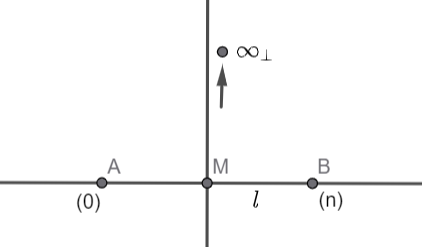
\includegraphics[width=0.5\textwidth]{kepek/kep5.png}
\end{figure}

Animation: $l$ and $A$ are fixed, $B$ moves on $l$ with degree $n$.

Calculate the degrees of the following objects one by one in this order:
\begin{itemize}
    \item $M$ (formula for the degree of the midpoint:
    $\deg M= \deg A+ \deg B - \#(A \text{ and } B \text{ are both ideal points})$)
    \item $\infty_{\perp}$
    \item the perpendicular bisector of $AB$
\end{itemize}

Solutions: ~\ref{sol_perpbs1}

\subsection{Ideal point of line}
\label{exc_idealpoint}

The ideal point $\infty_{l}$ of a line $l$ can be defined as the intersection of the ideal line and $l$. The ideal line is fixed, therefore the formula for the degree of intersection point gives

$$\deg \infty_{l}=\deg l - \#("l=\text{ideal line}")$$


Use this to calculate the degree of this ideal point:
\begin{figure}[H]
    %\centering
    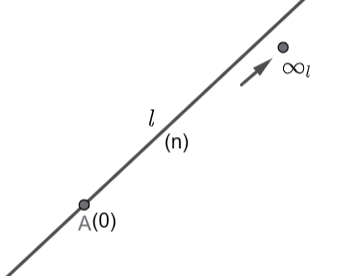
\includegraphics[width=0.4\textwidth]{kepek/kep5.5.png}
\end{figure}

Animation: $A$ is fixed, $l$ moves with degree $n$.
\begin{itemize}
    \item $\infty_l$
\end{itemize}


Solutions: ~\ref{sol_idealpoint}

\subsection{Perpendicular bisector 2}
\label{exc_perpbs2}

\begin{figure}[H]
    %\centering
    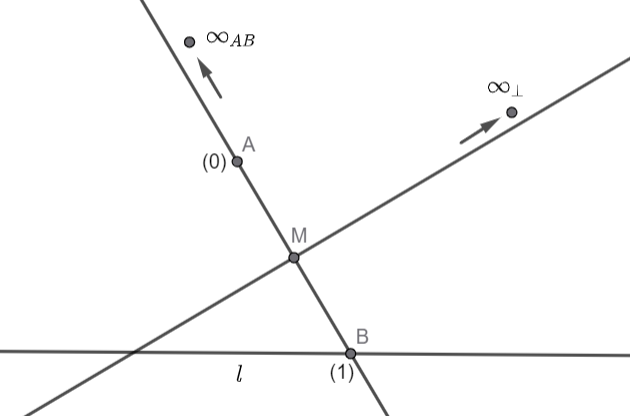
\includegraphics[width=0.6\textwidth]{kepek/kep6.png}
\end{figure}

Animation: $l$ and $A$ are fixed, $B$ moves on $l$ with degree $1$.

Calculate the degrees of the following objects one by one in this order:
\begin{itemize}
    \item $M$
    \item $\infty_{AB}$
    \item $\infty_{\perp}$
    \item the perpendicular bisector of $AB$
\end{itemize}

If $B$ is the ideal point, then what is the perpendicular bisector?

Solutions: ~\ref{sol_perpbs2}

% \subsection{Perpendicular bisector 3}
% \label{exc_perpbs3}

% \begin{figure}[H]
%     %\centering
%     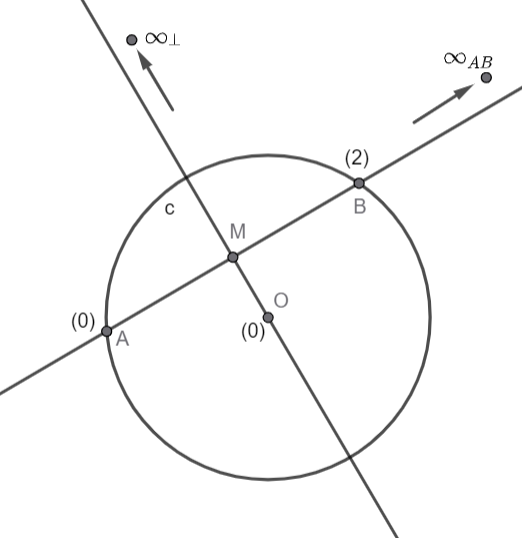
\includegraphics[width=0.5\textwidth]{kepek/kep7.png}
% \end{figure}

% Animation: $c$ and $A$ are fixed, $B$ moves on $c$ with degree 2.

% Calculate the degrees of the following objects one by one in this order:
% \begin{itemize}
%     \item $AB$
%     \item $\infty_{AB}$
%     \item $\infty_{\perp}$
%     \item $O$
%     \item the perpendicular bisector of $AB$ as line $O\infty_{\perp}$
%     \item $M$
%     \item the perpendicular bisector of $AB$ as line $M\infty_{\perp}$
% \end{itemize}

% The conclusion is that $M$ and $\infty_{\perp}$ coincide 2 times. This may seem impossible, but remember, that one has to check all the coincidences including complex times also. So they do coincide, when time is a complex number. To actually understand this, see chapter Circle points~\ref{cir}.

% Solutions: ~\ref{sol_perpbs3}

% \subsection{Circumcircle}

% \label{exc_circumcircle1}

% The degree of circumcircle is usually calculated by intersecting two perpendicular bisectors. Choose the two which have the lowest degree out of the three.

% \begin{figure}[H]
%     %\centering
%     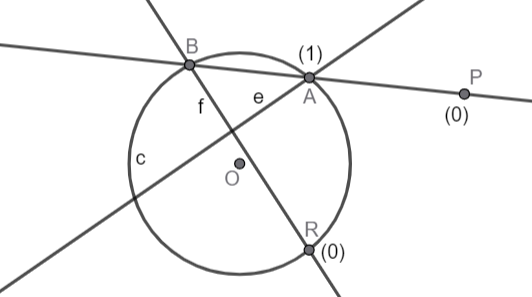
\includegraphics[width=0.6\textwidth]{kepek/kep8.png}
% \end{figure}

% Animation: $e$, $f$, $R$ and $P$ are fixed. $A$ moves on $e$ with degree 1.

% Calculate the degrees of the following objects one by one in this order:
% \begin{itemize}
%     \item $PA$
%     \item $B$
%     \item perpendicular bisector of $RA$
%     \item perpendicular bisector of $RB$
%     \item $O$
% \end{itemize}

% Solutions: ~\ref{sol_circumcircle1}

% \begin{exercise}[IMO SL 2005 G4]\label{exc_circumcircle2}
%     $AB$ and $CD$ are two segments with equal length. A variable point $X$ is on segment $AB$. $Y$ is on $CD$ such that $XA=YD$. The triangle formulated by lines $XY$, $AD$ and $BC$ has circumcenter $O$. Prove that $O$ moves on a line as $X$ varies.
% \end{exercise}

% \begin{figure}[H]
%     \centering
%     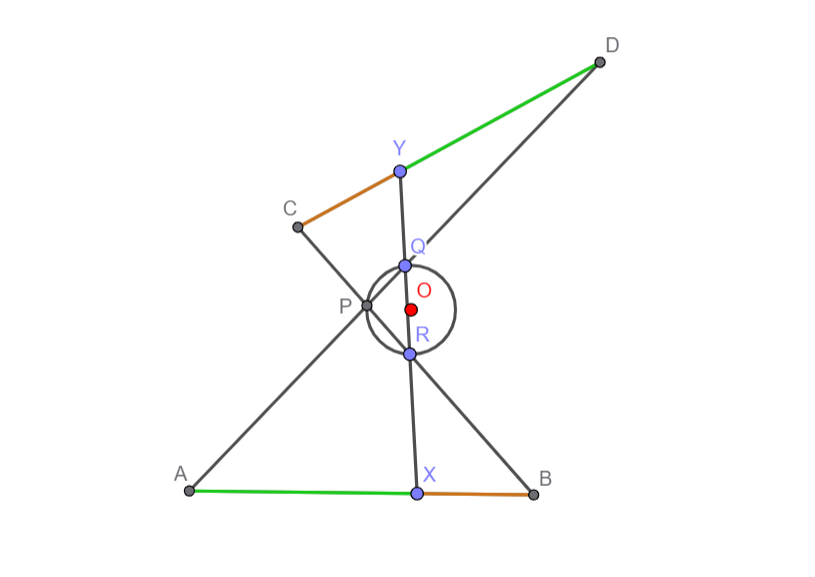
\includegraphics[width=0.8\textwidth]{kepek/kep9.png}
% \end{figure}

% Solution: ~\ref{sol_circumcircle2}

\subsection{Solutions}

(unfinished section)

\vspace{0.5cm}
\begin{minipage}{0.5\textwidth}
\subsubsection{Projection from line to line}
Exercise ~\ref{exc_linetoline}
\label{sol_linetoline}
\begin{itemize}
    \item $PA$ $(n)$
    \item $B$ $(n)$
\end{itemize}
$\deg (AB)= \deg (A) + \deg (B) - \# (A=B)$

$n=n+n-\# (A=B) \iff \# (A=B)=n$

Indeed, when $A=e\cap f$, then $B=e\cap f$ too, and $A$ and $B$ coincide. Since $A$ is a degree $n$ moving point on a degree 1 curve (line), $A$ goes through every point on the line exactly $n$ times including $e\cap f$. Therefore the number of coincidences is $n$.
\end{minipage}
\begin{minipage}{0.5\textwidth}
\subsubsection{Projection between line and conic}
Exercise ~\ref{exc_linetoconic}
\label{sol_linetoconic}
\begin{itemize}
    \item $PA$ $(n)$
    \item $B$ $(2n)$ By inverse Mászó-theorem we know that $\frac{\deg B+\deg A}{2}=\deg AB$. Therefore $\frac{\deg B+0}{2}=n\implies \deg B=2n$.
\end{itemize}
\end{minipage}

\vspace{1cm}
\begin{minipage}{0.5\textwidth}
\subsubsection{Projection from conic to itself} Exercise ~\ref{exc_conictoconic}
\label{sol_conictoconic}
\begin{itemize}
    \item $PA$ $(n)$
    \item $B$ $(n)$ By inverse Mászó-theorem
\end{itemize}
\end{minipage}
\begin{minipage}{0.5\textwidth}
\subsubsection{Perpendicular projection} Exercise ~\ref{exc_perpproj}
\label{sol_perpproj}
\begin{itemize}
    \item $\infty_{\perp}$ $(0)$
    \item $A\infty_{\perp}$ $(2)$
    \item $B$ $(2)$
\end{itemize}
\end{minipage}

\vspace{1cm}
\begin{minipage}{0.5\textwidth}
\subsubsection{Perpendicular bisector 1} Exercise ~\ref{exc_perpbs1}
\label{sol_perpbs1}
\begin{itemize}
    \item $M$ $(n)$
    \item $\infty_{\perp}$ $(0)$
    \item the perpendicular bisector of $AB$ $(n)$
\end{itemize}
\end{minipage}
\begin{minipage}{0.5\textwidth}
\subsubsection{Ideal point of line} Exercise ~\ref{exc_idealpoint}
\label{sol_idealpoint}
\begin{itemize}
    \item $\infty_l$ $(n)$
\end{itemize}
\end{minipage}

\vspace{1cm}
\begin{minipage}{0.5\textwidth}
\subsubsection{Perpendicular bisector 2} Exercise ~\ref{exc_perpbs2}
\label{sol_perpbs2}
\begin{itemize}
    \item $M$ $(1)$
    \item $\infty_{AB}$ $(1)$
    \item $\infty_{\perp}$ $(1)$
    \item the perpendicular bisector of $AB$ $(2)$
\end{itemize}
\end{minipage}
\begin{minipage}{0.5\textwidth}
\subsubsection{Perpendicular bisector 3} (exercise omitted from this draft)
\label{sol_perpbs3}
\begin{itemize}
    \item $AB$ $(1)$
    \item $\infty_{AB}$ $(1)$
    \item $\infty_{\perp}$ $(1)$
    \item $O$ $(0)$
    \item the perpendicular bisector of $AB$ as line $O\infty_{\perp}$ $(1)$
    \item $M$ $(2)$
    \item the perpendicular bisector of $AB$ as line $M\infty_{\perp}$ $(1)$
\end{itemize}
\end{minipage}

\subsubsection{Circumcircle}
\label{sol_circumcircle1}
(exercise omitted from this draft)
\begin{itemize}
    \item $PA$ $(1)$
    \item $B$ $(1)$
    \item perpendicular bisector of $RA$ $(2)$ This is the perpendicular bisector 2 case
    \item perpendicular bisector of $RB$ $(1)$ This is the perpendicular bisector 1 case
    \item $O$ $(2)$ Coincidence of the two bisectors happens when $A=e\cap f$.
\end{itemize}

\subsubsection{IMO SL 2005 G4}
\label{sol_circumcircle2}
Exercise ~\ref{exc_circumcircle2}

\section{Common animations}

The first step while using the Method of Moving Points is to find an appropriate animation of the figure. Here we list some of the most useful ones, but you should really be creative with these, because if you find a really good animation, it can save you lot of time.

Some general advise on finding the best animation: 
\begin{itemize}
    \item Try to fix circles as much as possible
    \item Avoid creating non polynomial points (see section Square root points~\ref{sqrt})
    \item Focus on the objects appearing in the statement, try to fix as much as possible.
    \item Fix 'busy' objects, that seem to have an important role in the problem
\end{itemize}

In this section, at each animation you have to calculate the degree of some objects to practice, and answer some questions. I advise you to have paper and pen with of you.

\subsection{Incircle animation}\label{incircleanim}

We used this one in the example problem too.

\begin{figure}[H]
    %\centering
    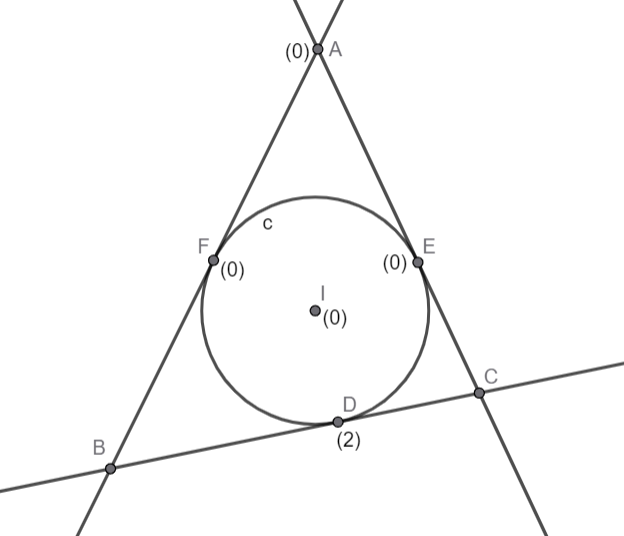
\includegraphics[width=0.6\textwidth]{kepek/kep10.png}
\end{figure}

Animation: $A$, $E$, $F$, $I$ and the incircle are fixed, $D$ moves on the incircle with degree 2.

Calculate the degrees of the following objects one by one in this order: 

\begin{itemize}
    \item $BC$
    \item $B$
    \item $C$
    \item $DE$
    \item $AD$
    \item $BI$
\end{itemize}


Often used special cases:
\begin{itemize}
    \item $D=E$ Where are points $A$ and $B$ in this case?
    \item $D=F$ Symmetric to the previous case
    \item $AB=AC$ This occurs when $BC$ is 'horizontal', either at the 'bottom' of the incircle, or at the 'top'. So there are two such cases.
    \item $D$ is the antipode of $E$, then $C$ is an ideal point.
    \item $D$ is the antipode of $F$, this is symmetric to the previous.
\end{itemize}


%oldaltörés


\begin{exercise}
    In triangle $ABC$, $D$, $E$ and $F$ are the tangency points of the incenter. $R$ is the intersection of $DI$ and $EF$. $M$ is the midpoint of $BC$. Show that $A, R, M$ are collinear.
\end{exercise}
\begin{figure}[H]
    \centering
    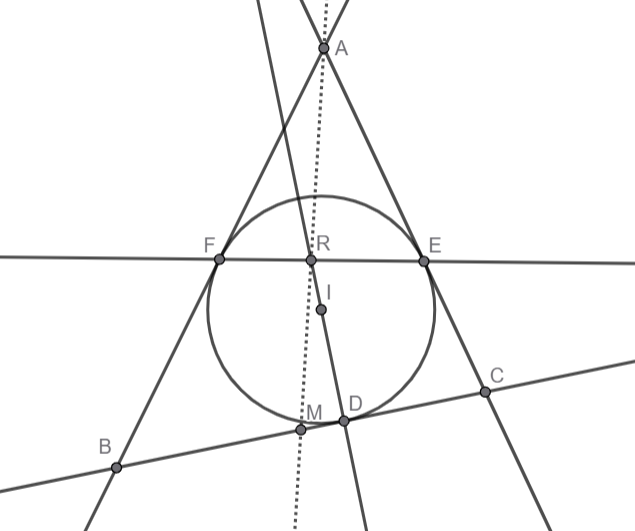
\includegraphics[width=0.6\textwidth]{kepek/kep11.png}
\end{figure}

\subsection{Circumcircle animation}

\begin{figure}[H]
    %\centering
    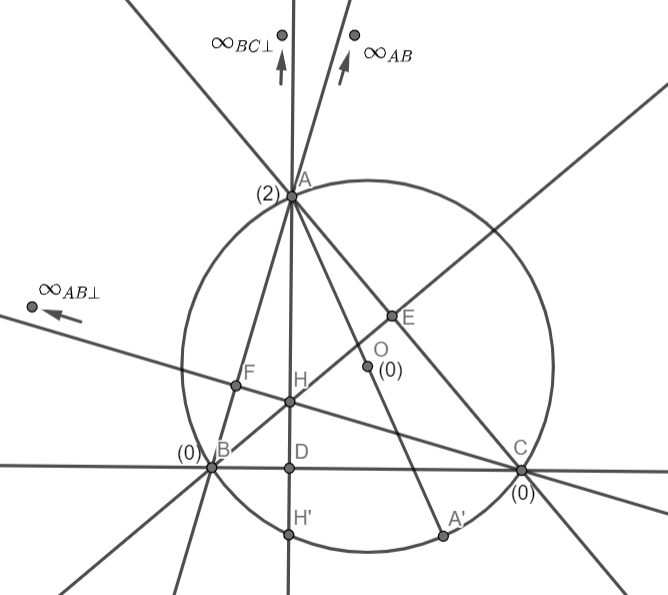
\includegraphics[width=0.7\textwidth]{kepek/kep12.png}
\end{figure}

Animation: $B$, $C$ and circumcircle are fixed, $A$ moves on the circumcircle with degree 2.

Calculate the degrees of the following objects one by one in this order: 

\begin{itemize}
    \item $AB$
    \item $AC$
    \item $\infty_{BC\perp}$ (the ideal point of the perpendicular direction to $BC$)
    \item the $A$-altitude
    \item $D$
    \item $\infty_{AB}$ (the ideal point of line $AB$)
    \item $\infty_{AB\perp}$ 
    \item $FC$
    \item $BE$
    \item $F$
    \item $E$
    \item $H$
    \item $H'$
    \item $AO$
    \item $A'$
\end{itemize}

What is the locus of
\begin{itemize}
    \item $F$
    \item $E$
    \item $H$
\end{itemize}

Often used special cases:
\begin{itemize}
    \item $AB=BC$. This happens when $A$ is at the 'bottom' or at the 'top' of the circumcircle, so there are two such cases.
    \item $A=B$. What is line $AB$ here, and where are points $E, F$ and $H$?
    \item $A=C$
    \item $A$ is the antipode of $C$. Where are points $F$ and $H$ in this case?
    \item $A$ is the antipode of $B$
    \item $A$ is one of the circle points (see chapter Circle points~\ref{cir})
\end{itemize}

\begin{exercise}
    Let $H$ be the orthocenter of acute triangle $ABC$, let $F$ be the foot of the altitude from $B$ to $AC$, and let $P$ be the reflection of $H$ across $AB$. Suppose that the circumcircle of triangle $CFP$ intersects line $AB$ at two distinct points $X$ and $Y$. Prove that $B$ is the midpoint of $XY$.
\end{exercise}

\subsection{Two sides of ABC is fixed}

\begin{figure}[H]
    %\centering
    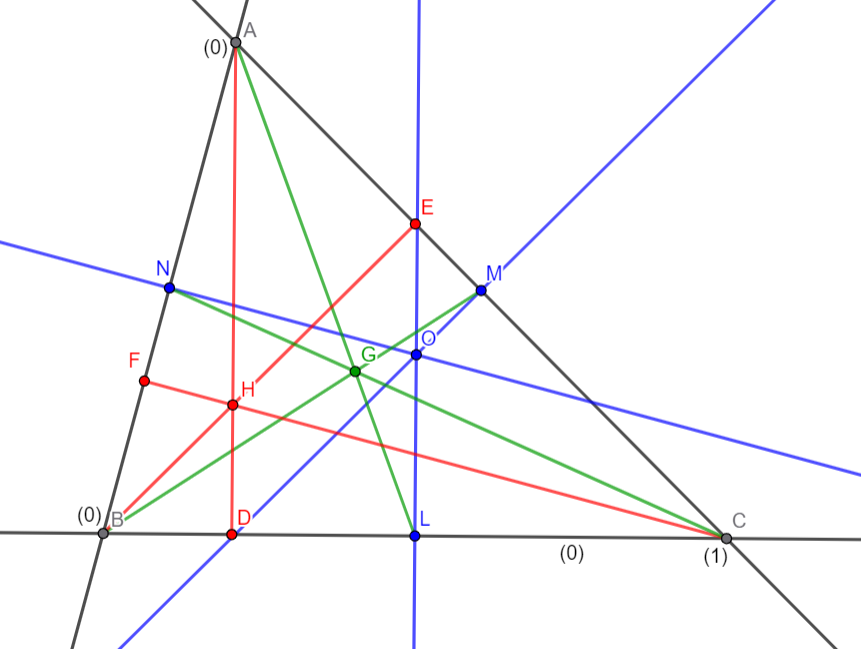
\includegraphics[width=0.8\textwidth]{kepek/kep12.5.png}
\end{figure}

Animation: $A$, $B$, $AB$ and $BC$ are fixed, $C$ moves on $BC$ with degree 1.

Useful when the circumcircle of $ABC$ isn't in the problem.

Calculate the degrees of the following objects one by one in this order: 

\begin{itemize}
    \item $AC$
    \item $AD$
    \item $D$
    \item $CF$
    \item $F$
    \item $BE$
    \item $E$
    \item $H$
    \item $L$
    \item $M$
    \item $N$
    \item $AL$
    \item $BM$
    \item $CN$
    \item $G$
    \item $LO$
    \item $MO$
    \item $NO$
    \item $O$
\end{itemize}

Often used special cases:
\begin{itemize}
    \item $CA=CB$ There's one such case
    \item $AB=AC$ There's one such case
    \item $BA=BC$ There's two such cases: when $C$ is on the right of $B$, and when it's on the left.
    \item $C=B$. What are points $H, G, O$ here?
    \item $C=\infty_{BC}$ What are points $H, G, O$ here?
    \item $C=D$. Now $ABC$ is right angled.
    \item $AB \perp AC$. $ABC$ is right angled in this case too.
\end{itemize}

\begin{exercise}[Euler line]
    Show that $H, G, O$ are collinear.
\end{exercise}

\begin{exercise}
    In triangle $ABC$ the feet of altitudes are $D$, $E$ and $F$ respectively on sides $BC$, $CA$ and $AB$.
    $EF$ intersects $BC$ at $P$, $FD$ intersects $AC$ at $Q$ and $DE$ intersects $AB$ at $R$. Show that $P$, $Q$ and $R$ lie on a line, and that this line is perpendicular to the Euler line of triangle $ABC$.
\end{exercise}

\begin{figure}[H]
    \centering
    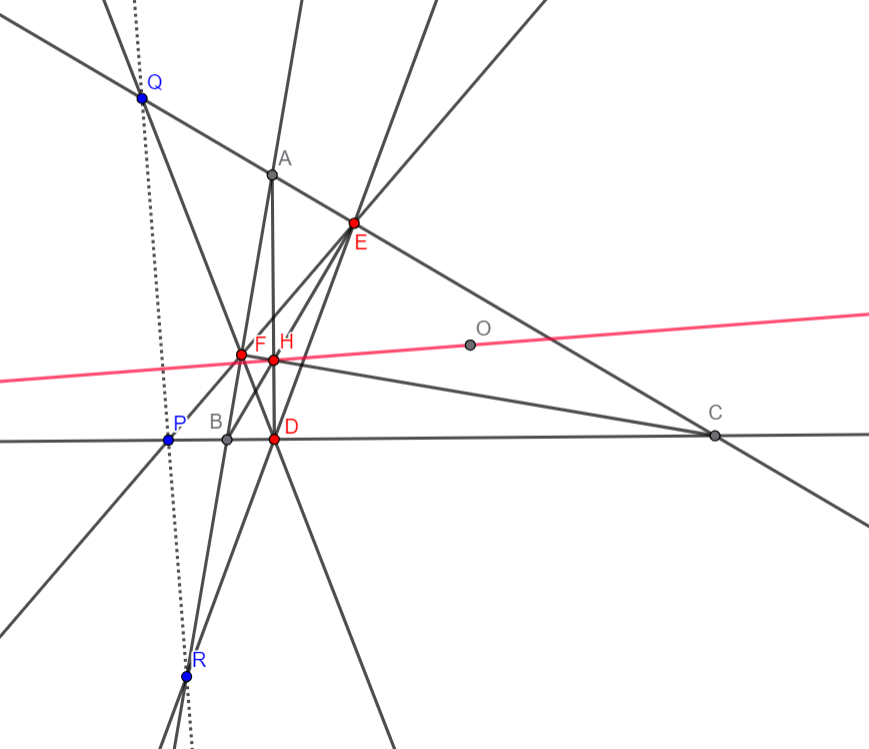
\includegraphics[width=0.9\textwidth]{kepek/kep13.png}
\end{figure}



\section{Circle points}\label{cir}

\subsection{Complex projective plane}

Until now we just accepted that every coordinate can be a complex number, but now we take massive advantage of this.

Every geometric statement is true over $\cc$ that is true over $\rr$, because usually these can expressed with coordinate geometry, which only uses addition, multiplication and division, so if such an expression is zero when substituting real numbers in, then it is also zero when substituting complex numbers.

Also everything 'exists' that may not exist over $\rr$, for example the two intersection point of a line far away and a circle, or the two tangents from an inner point of a circle.

% The following theorem underlies this intuition:

% \begin{theorem}[Bezout-theorem]
%     Let $f$ and $g$ be two algebraic curve with degree $a$ and $b$ on the complex projective plane. Then $f$ and $g$ has $a\cdot b$ intersection point (with multiplicity).
% \end{theorem}

\subsection{Properties}

\begin{definition}
    We call the points with homogeneous coordinates $(1:i:0)$ and $(1:-i:0)$ the two circle points, denoted with $\alpha_i$ and $\alpha_{-i}$
\end{definition}

These are the ideal points of the lines with slope $i$ and $-i$.

The natural definition of a circle on the complex projective plane is a conic in the following form:

$$Ax^2+Ay^2+Dxz+Eyz+Fz^2=0$$

If we divide by $A$, we get the usual equation of a circle.

\begin{lemma}
    Circles are exactly the conics that pass through the two circle points.
\end{lemma}
\begin{proof}
    A conic $Ax^2+Bxy+Cy^2+Dxz+Eyz+Fz^2=0$ passes through the two circle points $(1:i:0)$ and $(1:-i:0)$ if and only if
    $$A+iB-C=0\text{ and }A-iB-C=0\iff B=0, A=C$$
    which gives back the equation of a circle $Ax^2+Ay^2+Dxz+Eyz+Fz^2=0$.
\end{proof}

\begin{lemma}
    Every orientation-preserving homothety leaves the circle points fixed. Every orientation-reversing homothety swaps the circle points.
\end{lemma}
\begin{proof}
    An oriantation-preserving homothety can be expressed as the composition of rotation, translation, and scaling.
    
    Since the circle points are ideal points, scaling and translation keeps them in place.

    An angle $\varphi$ rotation takes a slope $s$ line to a slope $\frac{s+\tan \varphi}{1-s\cdot \tan \varphi}$ line by tangent addition formula. If $s=i$, this fraction is also $i$, and if it is $-i$, the fraction is also $-i$. So a rotation keeps both circle points in place.

    An orientation-reversing homothety can be expressed as the composition of an oriantation-preserving homothety and the mirroring with respect to the x-axis.

    The latter changes the sign of the y-coordinate of a point, while preserving the x-coordinate, so it swaps the circle points.
\end{proof}

\begin{lemma}
    Given a circle $\omega$ with center $O$. The two tangent lines from $O$ to $\omega$ are tangent to $\omega$ at the two circle points.
\end{lemma}
\begin{proof}
    If $O$ was an outer point, the two tangency point would lie on the polar of $O$. But now we are over $\cc$, so this reasoning works for $O$ too. The polar of $O$ is the ideal line, so the two tangency points are two ideal points. But the two ideal points of a circle are the two circle points.
\end{proof}

\begin{lemma}
    If $A$ and $B$ are two ideal points, and the angle between them is $\varphi$, then
    $$(A,B;\alpha_{i},\alpha_{-i})=e^{2i\varphi}$$
    So $A$ and $B$ correspond to perpendicular directions if and only if $(A,B;\alpha_{i},\alpha_{-i})=-1$, that is $A$, $B$ and $\alpha_{i}$, $\alpha_{-i}$ are harmonic.
\end{lemma}



\subsection{Circle points as special cases}

While animating a problem, if the initial point $X$ is moving on a circle, we can take the cases $X=\alpha_i$ and $X=\alpha_{-i}$. Then all the lines going through $X$ have slope i, moreover every line that is perpendicular to these have slope i. And it works with every angle, not just $90^{\circ}$. The mirror image of any of these lines however will have slope -i. It takes a while to get used to it, but once you're familiar with it, these become the simplest special cases. And also if $X=\alpha_i$ works, $X=\alpha_{-i}$ automatically works too.

For example at the circumcircle animation, if $A=\alpha_i$, then $BA$, $CA$ have slope $i$, so the perpendicular lines $BE$ and $CF$ also have slope i. This means that $F$, $E$ and $H$ are also at $\alpha_i$. Also line $AO$ is now tangent to the circumcircle, so $A'=A=\alpha_i$ But point $H'$, which is the mirror image of $H$ with respect to $BC$ is at $\alpha_{-i}$.

\begin{figure}[H]
    \centering
    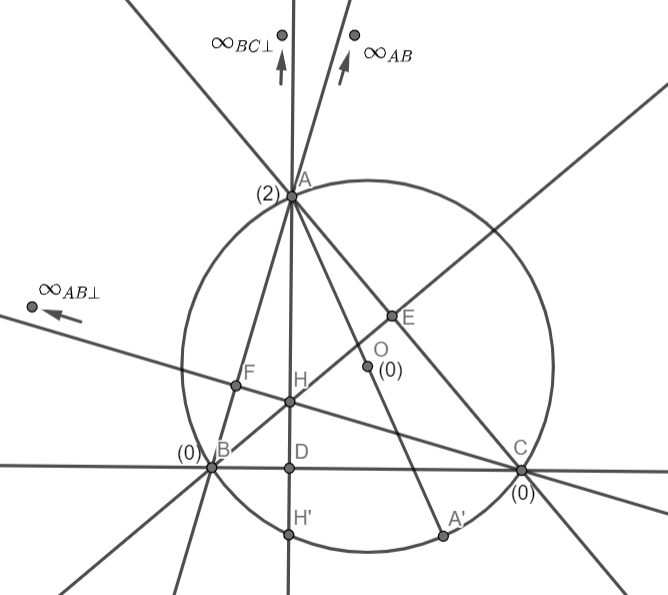
\includegraphics[width=0.7\textwidth]{kepek/kep12.png}
\end{figure}

\subsection{Coincidence at the circle points}

Often two points coincide at one of the circle points.

\begin{figure}[H]
    %\centering
    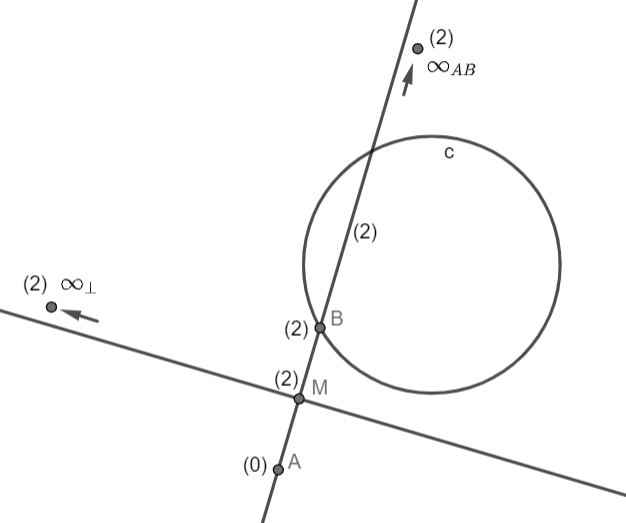
\includegraphics[width=0.6\textwidth]{kepek/kep14.png}
\end{figure}

Animation: $c$ and $A$ are fixed, $B$ moves on $c$ with degree 2.

We want to determine the degree of the perpendicular bisector of $AB$.

We calculate the degrees one by one:
\begin{itemize}
    \item $M$ is the midpoint of $A$ and $B$, and $A$ and $B$ are never ideal points at the same time, so $M$ has degree $0+2-0=2$.
    \item $AB$ has degree $0+2-0=2$
    \item $\infty_{AB}$ has degree 2
    \item $\infty_{\perp}$ has degree 2
    \item the perpendicular bisector of $AB$ is line $M\infty_{\perp}$, so it has degree $2+2-\#(M=\infty_{\perp})$. But when $B=\alpha_i$, $M$ is also $\alpha_i$, because $\alpha_i$ is an ideal point. Then $\infty_{AB}$ is also $\alpha_i$. But the perpendicular direction is also $\alpha_i$! So $M=\infty_{\perp}=\alpha_i$, and the same can be said when $B=\alpha_{-i}$. So the number of coincidences is 2, therefore the perpendicular bisector has degree $2+2-2=2$.
\end{itemize}
\begin{exercise}[Simson line]
    asd
\end{exercise}
\begin{exercise}[Droz-Farny line theorem]
    
\end{exercise}
\begin{exercise}[2025 China TST 1 day 1 problem 2]
    Suppose $\triangle ABC$ has $D$ as the midpoint of $BC$ and orthocenter $H$. Let $P$ be an arbitrary point on the nine point circle of $ABC$. The line through $P$ perpendicular to $AP$ intersects $BC$ at $Q$. The line through $A$ perpendicular to $AQ$ intersects $PQ$ at $X$. If $M$ is the midpoint of $AQ$, show that $HX \perp DM$.
\end{exercise}

\begin{exercise}[GIF 4.2.3]
    In triangle $ABC$, $H$ is the orthocenter. Take a line $l$ through $H$, and mirror it to the three sides of $ABC$. Prove that these lines are concurrent, and their intersection point lies on the circumcircle of $ABC$.
\end{exercise}

\section{Degree of angles}

We define degree for varying angles too.

\begin{definition}
    Let $\varphi(t)$ a time dependent angle.
    $\varphi(t)$ is polynomial if its tangent can be written as
    $$\tan \varphi(t)=\frac{p(t)}{q(t)}$$
    where $p$ and $q$ are polynomials of time with no common root.
    
    The degree of $\varphi$ is $\max (\deg p, \deg q)$
\end{definition}

\begin{remark}
    We consider directed angles modulo $180^\circ$.
\end{remark}

\subsection{Angle of a moving line}

Here is a useful point of view when considering an angle between lines. The ideal point of a line determines its direction, since all the lines going through one ideal point are parallel.

By fixing a "reference" direction we get a bijective correspondence between ideal points and angles, given by taking the directed angle between the direction of the ideal point and the reference direction.

\begin{lemma}
    Let $I$ be a polynomially moving ideal point, and $\alpha$ be the directed angle between the direction of $I$ and a fixed reference direction. Then $\alpha$ is a polynomial varying angle with the same degree as $I$. 
\end{lemma}
\begin{proof}
    We can suppose that the reference direction is horizontal.
    Let $I(t)=(p(t):q(t):0)$.
    Then $\tan \alpha(t)=\frac{q(t)}{p(t)}$, therefore $\alpha$ is polynomial with the same degree as $I$.
\end{proof}
\begin{example}
    Let $l$ be a degree $n$ line rotating around the origin. Then the angle between $l$ and the x-axis has degree $n$.
    \begin{proof}
        The ideal point $I$ of $l$ has degree $n-\#(\text{$l$ is the ideal line})=n$. Setting the horizontal x-axis as a reference direction, by the previous lemma the angle between $l$ and the x-axis has the same degree as $I$, which is $n$.
    \end{proof}
\end{example}
% \begin{lemma}
%     If $l$ is a polynomial moving line, and $\varphi$ is the signed angle between $l$ and the horizontal direction, then $\varphi$ is a polynomial angle with degree $\deg l - \#(l=\text{ideal line})=\deg \infty_l$
% \end{lemma}

% \begin{proof}
%     Let $O$ be the origin. Let $e$ be $O\infty_l$, this is the parallel line through the origin. It has degree $\deg \infty_l$.

%     If $\infty_l(t)=(p(t):q(t):0)$, then the slope of $e$ is $\frac{q(t)}{p(t)}$. So $\tan \varphi(t)=\frac{p(t)}{q(t)}$, therefore $\varphi$ is polynomial with the same degree as $\infty_l$
% \end{proof}

\subsection{Difference of angles}

To calculate the angle between two lines, we only have to consider the "angle between their ideal points", that is the difference of their angles with respect to a reference direction. Thus we need to calculate the degree of the difference of two angles:

\begin{theorem}
    Let $\alpha$ and $\beta$ be two polynomial angles. Then
    $$\deg (\alpha-\beta)=\deg \alpha + \deg \beta - \#(\tan\alpha = \tan \beta = i) - \#(\tan\alpha = \tan \beta = -i)$$
\end{theorem}
\begin{proof}
    $\tan(\alpha)=\frac{p}{q}$ and $\tan(\beta)=\frac{r}{s}$, so $p$ and $q$ are degree $\deg \alpha$ polynomials of time, and $r$ and $s$ are degree $\deg \beta$ polynomials of time.

    By the tangent addition formula $$\tan(\alpha-\beta)=\frac{\tan(\alpha)-\tan(\beta)}{1+\tan(\alpha)\tan(\beta)}=$$

    $$=\frac{\frac{p}{q}-\frac{r}{s}}{1+\frac{pr}{qs}}=\frac{ps-rq}{qs+pr}$$

These are $\deg \alpha + \deg \beta$ polynomials, but they may have common roots. So if $t_0 $ is a common root of both nominator and denominator, then $(t-t_0)$ can be factored out, and then simplifying by this term, we get rid of one common root, while lowering the degree of the polynomials by one. When applying this to all common roots, at the end $\deg (\alpha-\beta)=\deg \alpha + \deg \beta - \#(\text{nominator}=\text{denominator}=0)$
The latter is possible if $\tan(\alpha)-\tan(\beta)=0$ and $1+\tan(\alpha)\tan(\beta)=0$, so $\tan\alpha = \tan \beta = i$ or $\tan\alpha = \tan \beta = -i$.
\end{proof}

% Combining the previous two theorems, one can conclude the following:

% \begin{theorem}
%     If $e$ and $f$ are two moving lines with ideal points $\infty_e$, $\infty_f$, then the angle $\phi$ between them has degree

%     $$\deg(e)+\deg(f)-\# (e \text{ is ideal line})-\# (f \text{ is ideal line})- \# (\infty_e=\infty_f=\alpha_i)- \# (\infty_e=\infty_f=\alpha_-i)$$
% \end{theorem}

\begin{example}[Inscribed angle theorem]
    $A$ and $B$ are fixed points on a circle $\omega$, $X$ moves on $\omega$. Prove that the angle $AXB\angle$ is constant.
    \begin{proof}
        \begin{figure}[H]
            \centering
            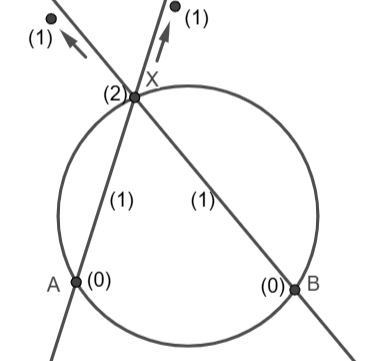
\includegraphics[width=0.5\textwidth]{kepek/kep14.5.png}
        \end{figure}
        Suppose $X$ moves on $\omega$ with degree 2. Then lines $AX$ and $BX$ has degree 1 by Mászó-theorem. Then their ideal points also have degree 1. Therefore their angles $\alpha$ and $\beta$ w.r.t the horizontal reference direction has degree 1 too. The difference of these two angles is $AXB\angle$. Now we use the previous theorem to calculate the degree of their difference:
        $$\deg AXB\angle=1+1-\#(\tan\alpha = \tan \beta = i) - \#(\tan\alpha = \tan \beta = -i)=1+1-2=0$$
        The reason we can reduce by 2 is that when $X=\alpha_i$, both ideal points of $AX$ and $BX$ are also $\alpha_i$, and therefore $\alpha$ and $\beta$ are angles between $\alpha_i$, and the horizontal direction, thus their tangents are both $i$. Same happens when $X=\alpha_{-i}$.
    \end{proof}
\end{example}
\subsection{Sum and multiple of angles}
\begin{theorem}
    Let $\alpha$ and $\beta$ be two polynomial angles. Then
    $$\deg (\alpha+\beta)=\deg \alpha + \deg \beta - \#(\tan\alpha = i \text{ and } \tan \beta = -i) - \#(\tan\alpha = -i \text{ and } \tan \beta = i)$$
\end{theorem}
\begin{proof}
    We apply the difference formula for $\alpha$ and $-\beta$.
\end{proof}

\begin{theorem}
    Let $\alpha$ be a polynomial angle, and $n$ a positive integer. Then
    $$\deg (n\cdot\alpha)=n\cdot \deg \alpha$$
\end{theorem}
\begin{proof}
    Let $A$ and $B$ be the ideal points corresponding to $\alpha$ and $n\cdot \alpha$ w.r.t. a reference direction respectively. Then $\deg A=\deg \alpha$ and $\deg B=\deg (n\cdot \alpha)$ While $\alpha$ rotates $180^{\circ}$, $n\cdot \alpha$ rotates $n\cdot 180^{\circ}$, so while $A$ goes through every point of the ideal line once, $B$ goes through every point $n$ times. Since a degree $n$ moving point on a fixed line goes through every point exactly $n$ times, $\deg B=n\cdot \deg A$. Therefore $\deg (n\cdot\alpha)=n\cdot \deg \alpha$
\end{proof}
\begin{remark}
    If $\tan \alpha=i$, then for any positive integer $n$, $\tan(n\alpha)=i$ also. For any negative integer $n$, $\tan(n\alpha)=-i$.
\end{remark}

\begin{exercise}[Geometry in figures 4.2.4]
    Triangle $ABC$ has circumcenter $O$. The mirror image of $BC$ w.r.t. $AB$ and the mirror image of $BC$ w.r.t $AC$ intersect at $X$. Prove that $A$, $O$ and $X$ are collinear.
\end{exercise}
\begin{proof}
        \begin{figure}[H]
            \centering
            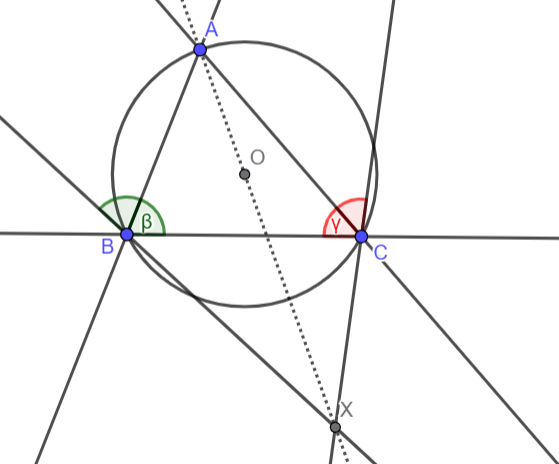
\includegraphics[width=0.5\textwidth]{kepek/kep14.6.png}
        \end{figure}
    We do the circumcircle animation, that is fix the circumcircle, $B$ and $C$, and animate $A$ on circumcircle with degree 2. Then $AB$ has degree 1 by Mászó-theorem, and it rotates around the fixed point $B$. $BC$ is fixed, so it can be taken as a reference direction, therefore $ABC\angle=\beta$ has degree $1$, just as line $AB$ has. Then by the previous theorem, $2\beta$ has degree 2. Line $BX$ has the same degree as $2\beta$, which is 2. Similarly line $CX$ has degree 2 too. Then their intersection $X$ has degree at most $2+2=4$. The statement $"A-O-X"$ has degree at most $2+0+4=6$. We have to find 7 cases:
    \begin{enumerate}
        \item $AB=AC$, when $A$ is at the top, true by symmetry
        \item $AB=AC$, when $A$ is at the bottom
        \item $A=B$, then one of the reflections of line $BC$ is $BC$ itself, the other is some random line through $B$, so $X$ is surely $B$. Then $A=X$, so $A$, $O$, $X$ are automatically collinear.
        \item $A=C$, same as previous case
        \item $A$ is the antipode of $B$. Then one of the reflections of line $BC$ is $BC$ itself, the other is some random line through $B$, so $X$ is surely $B$. Then $X$ and $A$ are antipodes, so $A-O-X$.
        \item $A$ is the antipode of $C$, same as previous
        \item $A=\alpha_i$. This means that $AB$ has slope $i$. Then $\tan \beta=i$, therefore by previous remark, $\tan (2\beta)=i$ too. So $BX$ is the line through $B$ with slope $i$. Similarly $CX$ is the line through $C$ with slope $i$. So their intersection $X$ is $\alpha_i$. Then $A=X$, so $A-O-X$ automatically.
    \end{enumerate}
\end{proof}


\begin{theorem}
    Let $\alpha$ and $\beta$ be two polynomial angles. Then the degree of the statement "$\alpha=\beta$" is exactly $\deg \alpha+ \deg \beta$.
\end{theorem}
\begin{proof}
    Let $A$ and $B$ be the ideal points corresponding to direction $\alpha$ and $\beta$ w.r.t. some reference direction. Then $\deg A= \deg \alpha$ and $\deg B=\deg \beta$. Now the statement "$\alpha=\beta$" is equivalent to the statement "$A=B$", which has degree $\deg A+\deg B$, since $A$ and $B$ move on a common fixed line, which is the ideal line.
\end{proof}


\subsection{Lines through a given point with given direction}

% If you have to measure angle $\alpha$ onto line $l$ from a point $P$ lying on $l$, you take $\infty_l$, measure $\alpha$ on it using the formula of the sum of angles, getting $\infty_{\text{new}}$, then take the line through $P$ and $\infty_{\text{new}}$. So you'll have to count the coincidences of $P$ and $\infty_{\text{new}}$.

A direction corresponds to an ideal point $I$, so to get a line through a given point $P$ with this direction, we just take the line through $P$ and $I$. Therefore to calculate the degree of the line, we have to use Zack's lemma. Notice that $P$ and $I$ can coincide only when $P$ is an ideal point.
\begin{example}
$P$ and $l$ are fixed, and $X$ moves on $l$ with degree 1.

The angle between $l$ and $PX$ is $\alpha$. If we measure $\alpha$ to $PX$ through $X$ once more, we get line $e$. We want to calculate the degree of $e$.

\begin{figure}[H]
    %\centering
    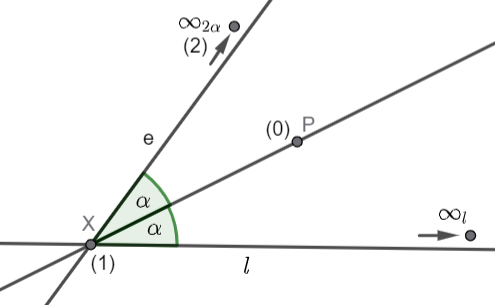
\includegraphics[width=0.5\textwidth]{kepek/kep15.png}
\end{figure}

The ideal point of $PX$ has degree 1. Since $l$ is fixed, it can be taken as a reference direction, so $\alpha$ has degree 1, just as the ideal point of $PX$.
Therefore $2\alpha$ has degree 2. 
$\infty_{2\alpha}$ is the ideal point corresponding to $2\alpha$, so it also has degree 2.
$e$ is the line through $X$ and $\infty_{2\alpha}$, so it has degree $1+2-1=2$, because $X$ and $\infty_{2\alpha}$ coincide once, when $X=\infty_l$ so $\alpha=0$, so $2\alpha$ is also 0, therefore $\infty_{2\alpha}=\infty_l=X$. So $e$ has degree 2.

\end{example}


\subsection{Angle bisector}

If $\alpha$ is a polynomial angle, then $\frac{\alpha}{2}$ is not necessarily polynomial. To resolve this, see chapter Square root points~\ref{sqrt}.
This means that the angle bisector of two polynomial lines are also not necessarily polynomial.

\subsection{Practice problems}

\begin{exercise}
    Let $ABCD$ be a square. Let $X$ be an arbitrary point on side $CD$. Line $e$ is the reflection of line $AB$ across the perpendicular bisector of $AX$. Let $Y$ be the intersection of $e$ and $BC$. What is the value of $XAY\angle$?
\end{exercise}



\section{Moving conics}

(unfinished section)

For further read see 
\url{https://www.researchgate.net/publication/398054957_Moving_conics_in_the_Method_of_Moving_Points}
\subsection{Degree of a moving conic}
We can define the degree of a moving conic too. Conics are uniquely determined by their 6 coefficients up to homogeneity, so a conic corresponds to a point in $\cc\pp^5$:

$$\{Ax^2+Bxy+Cy^2+Dxz+Eyz+Fz^2=0\} \leftrightarrow (A:B:C:D:E:F)$$

A moving conic is \textit{polynomial} if it corresponds to a polynomial moving point in $\cc\pp^5$.

The \textit{degree} of the polynomial moving conic is the degree of its corresponding point. In other words, a polynomial moving conic is defined by 6 polynomials (of time) as its coefficients $A,B,C,D,E,F$, such that the 6 polynomials do not have a common root. Then the degree of the moving conic is the maximum degree of the 6 polynomials.

We only consider the moving conics which are not always degenerate.

\subsection{Basic statements about moving conics}

\begin{theorem}
    Let $P$ be a polynomial moving point, and let $c$ be a polynomial moving conic. Then the degree of the statement "$P$ is on $c$" is
    $$2\deg P+ \deg c$$
\end{theorem}
\begin{proof}
    The point $P=(x:y:z)$ is on the conic $(A:B:C:D:E:F)$ iff
    $$Ax^2+Bxy+Cy^2+Dxz+Eyz+Fz^2=0$$
    This is a degree $2\deg P+ \deg c$ polynomial of time. Therefore it has exactly $2\deg P+ \deg c$ roots or it is constant zero.
\end{proof}

There is a unique conic through a general configuration of 5 points, so it is a reasonable statement that 6 points are on one conic.

\begin{theorem}\label{6onconic}
    Let $P_i$ $(i=1,\ldots ,6)$ be 6 polynomial moving points.
    Then the degree of the statement "The $P_i$ are on a conic" is 
    $$2\cdot \sum_{i=1}^6 \deg P_i$$
\end{theorem}
\begin{proof}
The 6 points are on a conic if and only if
   $$ \det
\begin{pmatrix}
x_1^2 & x_1 y_1 & y_1^2 & x_1 z_1 & y_1 z_1 & z_1^2 \\[4pt]
x_2^2 & x_2 y_2 & y_2^2 & x_2 z_2 & y_2 z_2 & z_2^2 \\[4pt]
x_3^2 & x_3 y_3 & y_3^2 & x_3 z_3 & y_3 z_3 & z_3^2 \\[4pt]
x_4^2 & x_4 y_4 & y_4^2 & x_4 z_4 & y_4 z_4 & z_4^2 \\[4pt]
x_5^2 & x_5 y_5 & y_5^2 & x_5 z_5 & y_5 z_5 & z_5^2 \\[4pt]
x_6^2 & x_6 y_6 & y_6^2 & x_6 z_6 & y_6 z_6 & z_6^2
\end{pmatrix}
= 0$$
If we expand the determinant, we see that it is a degree $2\cdot \sum_{i=1}^6 \deg P_i$ polynomial of time.
\end{proof}

Similarly to points and lines, projective transformations preserve moving conics' degree.
\begin{theorem}
    Let $c$ be a polynomial moving conic. Then the image of $c$ with respect to a fixed projective transformation is also a polynomial moving conic with degree $\deg c$.
\end{theorem}

\subsection{Conic through 5 points}

There are three types of conics in terms of degeneracy:
\begin{itemize}
    \item Non-degenerate: The usual conic that one imagines.
    \item Union of two different lines: This is also a conic, since if you multiply the equation of two lines, and expand the parentheses, you get a conic equation.
    \item One line counted twice: if you take the square of the equation of a line, it is also a conic equation
\end{itemize}

We know that there is a conic through a general configuration of 5 points, but what can be said if the 5 points are in a very unfortunate position?

First look at the case, when 3 points out of the 5 are collinear on a line $l$. Then the conic through them must contain $l$ as a component (in other words, as a subset). So the conic must be the union of two lines, therefore the other line is the line through the remaining 2 points. So in this case the conic is still unique.

%picture about this

Let's look at other cases. There always exists a conic through 5 points, no matter how degenerate their position is, however, it may not be unique. In fact, it is not unique if either "2 points coincide", or "4 points are on a line", otherwise the conic is unique. Indeed, if (at least) 2 points coincide, then there are infinitely many conics through (at most) 4 points. And if (at least) 4 points lie on a common line $l$, then the conic can be the union of $l$ and any line through the 5th point.

%picture about these

With this in mind the following proposition is not that surprising.

\begin{theorem}\label{conicthr5}
    Let $P_1$, $P_2$, $P_3$, $P_4$ and $P_5$ be five polynomial moving points. Then the conic $c$ always going through them is polynomial, and its degree is at most
    $$\deg c= 2\cdot\sum_{i=1}^5\deg P_i-\#(\text{"any two points are the same" or "any 4 points are collinear"})$$
\end{theorem}
\begin{remark}
    The $\#$ part is taken with multiplicity. A lower bound to the multiplicity (which upper bounds the degree of the conic) is 5-(number of different points among the 5), so for example if 3 points coincide, the multiplicity is at least 2.
\end{remark}

\begin{example}
    something
\end{example}

\subsection{Moving circles}

Recall that a circle is a conic which passes through the two circle points $\alpha_i$ and $\alpha_{-i}$.

If we take a special case of the previous theorem with fixing the moving points $P_4$ and $P_5$ at $\alpha_i$, $\alpha_{-i}$ respectively, we get the following (make sure to think it through why):

\begin{theorem}
    Let $P_1$, $P_2$ and $P_3$ be three polynomial moving points. Then their circumcircle $c$ is polynomial, and its degree is at most
    $$\deg c= 2(\deg P_1+\deg P_2+\deg P_3)-\#(\text{"any two points are the same" or "a point is one of the circle points"}$$
    $$\text{or "any 2 points are on the ideal line" or "all 3 points are collinear on a line with slope $i$ or $-i$"})$$
\end{theorem}

\begin{example}
    Let $c$ be a circle, $A$ a fixed point on $c$, $B$ a fixed point not on $c$ and $C$ a degree 2 moving point on $c$. (Imagine the movement!) What is the degree of circle $(ABC)$? 
    Apply the previous formula:
    $$\deg (ABC)=2(0+0+2)-3=1$$
    We can reduce the degree 3 times (which means at least one of the events inside the $\#$ part is satisfied), first when $C=A$, then two points are the same, then two times when $C=\alpha_i$ and $C=\alpha_{-i}$, because one of the points is a circle point. $C$ will be the circle points because $C$ moves on a circle.
\end{example}
\begin{remark}
    There are cases when more than one event is satisfied, however this does not guarantee multiplicity more than 1, most of the times we can still only reduce the degree by 1.
\end{remark}
\begin{example}
    Fixed lines $e$ and $f$ intersect in fixed point $A$. Two moving points $B$ and $C$ are moving with degree 1 on $e$ and $f$ respectively such that line $BC$ has constant direction, that is it passes through a fixed ideal point $I$. (Imagine the movement!) What is the degree of circle $(ABC)$?
    Apply the formula:
    $$\deg (ABC)=2(0+1+1)-3=1$$
    We can reduce the degree 3 times, first when $A=B=C$, here recall that if 3 points coincide out of the five points $A$, $B$, $C$, $\alpha_i$, $\alpha_{-i}$, we can reduce by 2. Then when $A$ and $B$ both become ideal points at the same time, we can reduce by 1.
\end{example}
\begin{exercise}
    What is the degree of the circle $(ABC)$ at the incircle animation? ~\ref{incircleanim}
\end{exercise}
\begin{exercise}
    Let $ABC$ be an acute triangle, and $X$ and $Y$ points on sides $AB$ and $AC$ respectively, such that $BX=CY$. Let $M$ be the midpoint of longer arc $BAC$ on the circumcircle of $ABC$. Prove that the circumcircle of $AXY$ passes through $M$.
\end{exercise}

\begin{exercise}[Towards proving that the 9 point circle is tangent to the incircle]
    The 9 point circle of a triangle $ABC$ is the circle passing through the midpoints and feet of perpendiculars of all sides.
    What is the degree of the 9 point circle of $ABC$ at the incircle animation? (Hint: Define it to be the circle through this three points: the feet of perpendicular from $B$, the feet of perpendicular from $C$ and the midpoint of $AB$)

\end{exercise}

We discussed the degree of statement that 6 points are on a conic, now take a special case of this, when $P_5=\alpha_i$ and $P_6=\alpha_{-i}$ (fixed points), and conclude the following:
\begin{theorem}
    Let $P_i$ $(i=1,2,3,4)$ be 4 polynomial moving points.
    Then the degree of the statement "The $P_i$ are on a circle" is 
    $$2\cdot \sum_{i=1}^4 \deg P_i$$
\end{theorem}

The next theorem tells us the degree of the center of a moving circle (not true for general conics!)

\begin{theorem}
    Let $c$ be a polynomial moving circle. Then its center $O$ is a polynomial moving point with degree at most

    $$\deg O=\deg c-\#(c=\text{ideal line counted twice})$$
\end{theorem}
\begin{example}
    $"c=\text{ideal line counted twice}"$ is equivalent to $c$ not having finite (not ideal) points. Therefore if $c$ has a fixed finite point, then we can never reduce degree, so $\deg c=\deg O$.
\end{example}

By rearranging the theorem, we get
$$\deg c=\deg O+ \#(c=\text{ideal line counted twice})$$
We can use this to calculate the degree of the circle by knowing the degree of its center, but this time the $\#(...)$ part is with a $+$ sign, therefore we have to tell the exact multiplicity of the event happening, here is how:
\begin{remark}
    The multiplicity of $\#(c=\text{ideal line counted twice})$ is ... something idk
\end{remark}
\begin{example}
    Let $O$ be a degree 1 moving point and $c$ a circle with center $P$ and fixed radius. Apply the rearranged formula to get
    $$\deg c=\deg O+ \#(c=\text{ideal line counted twice})=1+1=2$$
    "$c=\text{ideal line counted twice}$" happens once when $O$ is ideal point, since then $c$ has no finite point. And it happens with with multiplicity 1, since ...????
\end{example}
\begin{exercise}
    What is the degree of the circumcenter of $ABC$ at the incircle animation? ~\ref{incircleanim}
\end{exercise}

\subsection{Degree 1 and 2 circles}
\begin{lemma}
    A degree 1 circle's positions as time varies form a pencil of circles, meaning there exists a common radical axis of all positions of $c$.
\end{lemma}


\begin{exercise}[IMO SL 2005 G4]\label{exc_circumcircle2}
    $AB$ and $CD$ are two segments with equal length. A variable point $X$ is on segment $AB$. $Y$ is on $CD$ such that $XA=YD$. The triangle formulated by lines $XY$, $AD$ and $BC$ has circumcenter $O$. Prove that $O$ moves on a line as $X$ varies.
\end{exercise}
\begin{figure}[H]
    \centering
    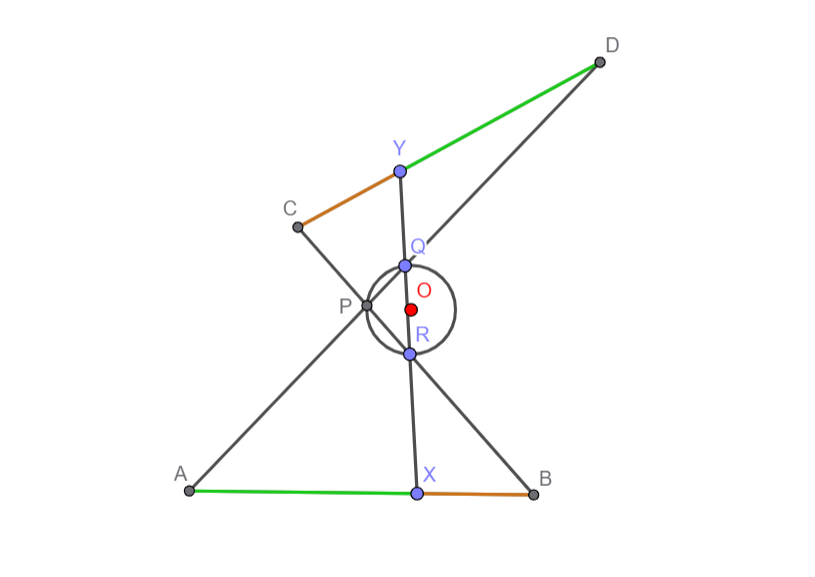
\includegraphics[width=0.8\textwidth]{kepek/kep9.png}
\end{figure}

Solution: ~\ref{sol_circumcircle2}

\begin{exercise}[Iranian Geometry Olympiad 2024 Advanced P5, le kéne ellenőrizni, hogy ez mennyire nehéz]
    Cyclic quadrilateral $ABCD$ with circumcircle $\omega$ is given. Let $E$ be a fixed point on segment $AC$. $M$ is an arbitrary point on $\omega$, lines $AM$ and $BD$ meet at a point $P$. $EP$ meets $AB$ and $AD$ at points $R$ and $Q$, respectively, $S$ is the intersection of $BQ,DR$ and lines $MS$ and $AC$ meet at a point $T$. Prove that as $M$ varies the circumcircle of triangle $\bigtriangleup CMT$ passes through a fixed point other than $C$.
\end{exercise}

\begin{lemma}
    A degree 2 circle's positions as time varies have a common radical center.
\end{lemma}
\begin{exercise}[USA TST 2021 P2]
    Points $A$, $V_1$, $V_2$, $B$, $U_2$, $U_1$ lie fixed on a circle $\Gamma$, in that order, and such that $BU_2 > AU_1 > BV_2 > AV_1$.

Let $X$ be a variable point on the arc $V_1 V_2$ of $\Gamma$ not containing $A$ or $B$. Line $XA$ meets line $U_1 V_1$ at $C$, while line $XB$ meets line $U_2 V_2$ at $D$. Let $O$ and $\rho$ denote the circumcenter and circumradius of $\triangle XCD$, respectively.

Prove there exists a fixed point $K$ and a real number $c$, independent of $X$, for which $OK^2 - \rho^2 = c$ always holds regardless of the choice of $X$.
\end{exercise}


\subsection{Intersection of conics}

According to Bezout's theorem, a degree $a$ and a degree $b$ algebraic curve in $\cc\pp^2$ which don't have a common component (an algebraic curve contained in both) have exactly $ab$ intersection points counted with multiplicity. As special cases, a line and a conic have two intersection points (with mul) and two conics have four.

The two intersection points of a moving conic and a moving line are not necessarily polynomial, but they are square root points (see chapter ~\ref{sqrt}). However, if one of them is polynomial, then the other must be polynomial too. In either case we can calculate the sum of their degrees.

\begin{theorem}
    Let $l$ be a polynomial moving line and let $c$ be a polynomial moving conic. Then their 2 intersection points $A,B$ form a square root point pair with degree
    $$2\deg (A,B)= \deg c + 2\deg l-\#(\text{$c$ contains $l$ as a component})$$
\end{theorem}
\begin{example}
    If $c$ is fixed, then the two intersection points $A$, $B$ will be a square root pair with degree
    $$2\deg(A,B)=\deg c + 2\deg l-\#(\text{$c$ contains $l$ as a component})=0+2\deg l+0$$
    The $\#$ part is 0 since $l$ can only be a component of $c$ if $c$ is degenerate, but $c$ is a fixed nondegenerate conic.
    
    Therefore the average degree of the pair $(A,B)$ is
    $$\deg(A,B)=\deg l$$
\end{example}
\begin{remark}
    If one of $A$, $B$ is polynomial, then the other is so, and the formula with polynomial degrees is
    $$\deg A+\deg B= \deg c + 2\deg l-\#(\text{$c$ contains $l$ as a component})$$
\end{remark}
\begin{example}
    Let $A$, $B$ be fixed points and $l$ a fixed line through $A$. Let $C$ be a degree 1 moving point on $l$. Let $e$ be a line through $C$ with fixed direction. Let $D$ be the intersection of $e$ and circle $(ABC)$. What is the degree of $D$?

    First of all $e$ has degree 1, and $(ABC)$ has degree 1 too. Then their intersection points are $C$ and $D$. Since $C$ is polynomial, $D$ is polynomial too. Then the sum of their degree is
    $$\deg C+\deg D=\deg (ABC)+2\deg (e)-\#(\text{$(ABC)$ contains $e$ as a component})=1+2\cdot 1-1=2$$
    $(ABC)$ contains $e$ as a component when $C$ is the ideal point, because then $(ABC)$ is the union of the ideal line and $AB$, and $e$ is the ideal line. Since $\deg C=1$, we have
    $$\deg D=2-1=1$$

    I always forget to subtract the degree of the OTHER intersection point (this last step), so be more cautious than me, and remember it :D
\end{example}

\begin{exercise}
    What is the degree of the arc midpoint of $BC$ opposite to $A$ at the incircle animation ~\ref{incircleanim}? Define it to be the intersection of the $A$-angle bisector and the circumcircle $(ABC)$.
\end{exercise}

\begin{exercise}
    Let $ABC$ be a triangle, and $D$ a point on side $BC$. The second intersection point of circle $(ABD)$ with $AC$ is $E$. The second intersection point of $(ACD)$ with $AB$ is $F$. Show that the line through $D$ perpendicular to $BC$ passes through the center of circle $(AEF)$.
\end{exercise}

Two circles have four intersection points, among which two are the circle points. We can think of the other two intersection points separately.

\begin{theorem}
    Let $c_1$ and $c_2$ be two polynomial moving circles. Then their two intersection points $A,B$ (besides the two circle points) form a square root point pair with degree
    $$2\deg (A,B)=2\deg c_1 + 2\deg c_2-\#(\text{$c_1$ and $c_2$ have a common component})$$
\end{theorem}
\begin{remark}
    The multiplicity of $\#(\text{$c_1$ and $c_2$ have a common component})$ at $t_0$ is at least 2 if $c_1=c_2$ at $t_0$.
\end{remark}
\begin{example}
    Let $c$ be a fixed circle and $d$ be a degree 2 polynomial moving circle, which coincides with $c$ one time along its movement. Then their two intersection points $A$, $B$ (besides the two circle points) have degree
    $$\deg (A,B)=2\cdot 0+2\cdot 2 - 2=2$$
    As the remark stated, if the two circles coincide (or equivalently they have a degree 2 common component), then the multiplicity of \#(\text{$c_1$ and $c_2$ have a common component}) is at least 2.
\end{example}
\begin{remark}
    If one of $A$, $B$ is polynomial, then the other is so, and the formula with polynomial degrees is
    $$\deg A+\deg B= 2\deg c_1 + 2\deg c_2-\#(\text{$c_1$ and $c_2$ have a common component})$$
\end{remark}


\begin{example}
    Let $c$ be a fixed circle and $A$ be a fixed point on it. A degree 1 circle $d$ through $A$ intersects $c$ at $B$. What is the degree of $B$?

    First of all, since $A$ is fixed, it is polynomial, therefore the other intersection point $B$ will be polynomial too.

    The sum of their degree is
    $$\deg A+\deg B=2\cdot 0+2\cdot 1-0=2$$

    Since $\deg A=0$, it follows that $\deg B=2$.
\end{example}

\begin{exercise}
    We have a fixed triangle $ABC$ with circumcircle $\omega$ and a degree 1 moving point $P$ along a random line $l$. Line $BP$ meets side $AC$ at $Y$ while line $CP$ meets side $AB$ at $X$. Let $Q$ be the second intersection of $\omega$ and the circumcircle of triangle $AXY$. Let $K$ be the second intersection of ray $AP$ and $\omega$. Prove that as $P$ varies, the circumcircles of triangle $QPK$ all have a common radical center.
\end{exercise}
\begin{exercise}[2019 APMO P3, nehézséget le kell még ellenőrizni, meg megoldani a feladatot]
    Let $ABC$ be a scalene triangle with circumcircle $\Gamma$. Let $M$ be the midpoint of $BC$. A variable point $P$ is selected in the line segment $AM$. The circumcircles of triangles $BPM$ and $CPM$ intersect $\Gamma$ again at points $D$ and $E$, respectively. The lines $DP$ and $EP$ intersect (a second time) the circumcircles to triangles $CPM$ and $BPM$ at $X$ and $Y$, respectively. Prove that as $P$ varies, the circumcircle of $\Delta AXY$ passes through a fixed point $T$ distinct from $A$.
\end{exercise}

Similarly we can calculate the sum of degrees of the 4 intersection points of two conics:

\begin{theorem}
    Let $c_1$ and $c_2$ be two polynomial moving conics. Then their 4 intersection points $A,B,C,D$ are not necessarily polynomial, but if they are, then
    $$\deg A+\deg B+\deg C+\deg D =2\deg c_1 + 2\deg c_2-\#(\text{$c_1$ and $c_2$ have a common component})$$
\end{theorem}
\begin{remark}
    The multiplicity of $\#(\text{$c_1$ and $c_2$ have a common component})$ is at least the degree of the common component as an algebraic curve. This means that if $c_1=c_2$, then their common component is the whole conic, this has degree 2, so we can reduce the degree by 2.
\end{remark}
\begin{proof}
    I don't know yet
\end{proof}
\begin{example}
    
\end{example}

\subsection{Tangency}

\begin{theorem}
    Let $l$ be a polynomial moving line, and let $c$ be a polynomial moving conic. Then the degree of the statement "$l$ is tangent to $c$" is 
    
    $$2\deg l+ 2\deg c$$
\end{theorem}
\begin{remark}

    Here "$l$ is tangent to $c$" is true iff either one of the following is true:
\begin{itemize}
    \item The conic is nondegenerate, and $l$ is tangent to it in the normal sense
    \item The conic splits into two different lines, and $l$ goes through the intersection point of the two lines
    \item The conic is a single line counted twice, in this case every line $l$ is tangent to it.
\end{itemize}
\end{remark}
\begin{example}
    Let $l$ be a degree 2 moving line. Then $l$ is always tangent to a conic.

    \begin{proof}
        Take $5$ positions of $l$, there is a conic $c$ tangent to all of them. Then the statement "$l$ is tangent to $c$" has degree $2\cdot 2+2\cdot 0=4$. But it is true 5 times, therefore it is always true, so $l$ is always tangent to $c$.
    \end{proof}
\end{example}


\begin{theorem}
    Let $c_1$ and $c_2$ be two polynomial moving circles. Then the statement "$c_1$ and $c_2$ are tangent" has degree
    $$2\deg c_1 + 2\deg c_2$$
\end{theorem}
\begin{remark}
    Here "$c_1$ and $c_2$ are tangent" is true iff either one of the following is true:
    \begin{itemize}
        \item $c_1$ and $c_2$ does not have common component, thus they have four intersection points $A$, $B$, $\alpha_i$ and $\alpha_{-i}$ (which are possibly the same) and $A=B$.
        \item $c_1=c_2$
        \item If $c_1$ and $c_2$ has a common line component, which is not the ideal line
        \item If $c_1$ and $c_2$ has a common line component, which is the ideal line, and their other line components intersect on the ideal line.
    \end{itemize}
\end{remark}

%impossible to find a last case
% \begin{exercise}[after concyclic statement]
%     Let $ABC$ be a triangle with $AB=AC$, and let $M$ be the midpoint of $BC$. Let $P$ be a point such that $PB<PC$ and $PA$ is parallel to $BC$. Let $X$ and $Y$ be points on the lines $PB$ and $PC$, respectively, so that $B$ lies on the segment $PX$, $C$ lies on the segment $PY$, and $\angle PXM=\angle PYM$. Prove that the quadrilateral $APXY$ is cyclic.
% \end{exercise}





\begin{example}
    The 9 point circle is tangent to the incircle.

    \begin{proof}
        We use the incircle animation, and in a previous exercise we saw that the 9 point circle has degree 2. The incircle is fixed, so the statement has degree $2\cdot 2+2\cdot 0=4$, so we need 5 cases. If $ABC$ is isosceles we are done by symmetry reasons, we have 4 such cases (two when $AB=AC$, one when $BA=BC$ and one when $CA=CB$). The 5th case is when $B$ is an ideal point. Here the 9 point circle degenerates into the union of line $NR$ and the ideal line. We are left to prove a simple elementary problem.
        \begin{figure}[H]
        \centering
        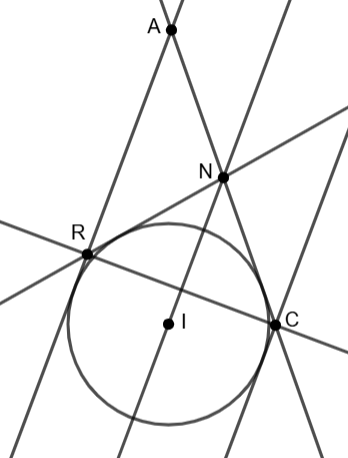
\includegraphics[width=0.25\textwidth]{kepek/feuerbach2.png}
        \end{figure}
        Now $AB$ and $CB$ are parallel lines. Let the parallel line halfway between them be $l$. $N$ is the midpoint of $AC$, so it is on $l$. $I$ is the center of the incircle, which is tangent to both $AB$ and $CB$, so $I$ is also on $l$. $R$ is the foot of the altitude from $C$ to $AB$, now this is the mirror image of $C$ w.r.t. $l$. Therefore segments $NC$ and $NR$ are also mirror images w.r.t. $l$. Since $NC$ is tangent to the incircle, $NR$ must be tangent to it too. But line $NR$ is the degenerate 9 point circle, so we proved the statement.
    \end{proof}
\end{example}

\section{Animation inside animation}

Suppose that in a geometry problem, the initial moving point $A$ has a logical symmetric pair $B$. This means that swapping the role of $A$ and $B$ doesn't change the problem. 

We want to solve the problem by animating $A$ and fixing $B$, and let's say we need $n$ special cases to prove it.

Suppose we want to prove the special case when $A=X$, where $X$ is a certain position on the locus of $A$. The trick is the following: We can prove this case by using MMP, animating $B$ and fixing $A$ at $X$ so that this animation is logically symmetric to the original animation. This way we need the same number of special cases, furthermore we can reuse all the previously proven special cases by symmetry.

This is especially useful while finding the last special case. Suppose we already proved $n-1$ cases, and we would like to find the last one. We can put $A$ in any position $X$, and prove the case $A=X$. To do this we use MMP, and animate $B$. This animation is logically symmetric to the original, therefore we can reuse all $n-1$ special cases that we already proved, by symmetry, and we only need 1 more special case. So we can also put $B$ in any position $Y$, making sure that the case $B=Y$ is different from the previous $n-1$ cases, and then prove the statement when $B=Y$.

This way we could specify the position of both $A$ and $B$ at the last case, we only need to pay attention not to reuse a previous case.

And if there are more than two symmetric points, we can specify all of them for the last case with the same logic.

\begin{example}
        
\end{example}

It's super easy to forget about this when you just can't find that last case, so here is a message for the future you: If your stuck with the last case, use animation inside animation!

\section{Inversion}

Inversion comes up fairly often in geometry problems, so here's how to handle it.

\begin{theorem}
    Let $\omega$ be a circle with center $O$, and $P$ a polynomial moving point. The inverse image of $P$ with respect to $\omega$ is $Q$. $\alpha_i$ and $\alpha_{-i}$ are the two circle points. Then
    $$\deg Q=2\cdot \deg P - \#(P=O) - \#(P=\alpha_i) - \#(P=\alpha_{-i})$$ (with multiplicity)
\end{theorem}

\begin{proof}
    We can suppose that $\omega$ is the unit circle centered at the origin.
    $$P=(x:y:z)$$
    After some calculations
    $$Q=(xz:yz:x^2+y^2)$$
    The coordinates are degree $2\cdot \deg P$ polynomials of time, so now we only have to subtract the number of times when $(xz:yz:x^2+y^2)=(0:0:0)$. This is because if at a time $t_0$ all three polynomials are zero, then we can factor out $(t-t_0)$ from them, then divide with it. After we do this with all common roots, the degree drops by the number of common roots.

    $(xz:yz:x^2+y^2)=(0:0:0)$ can happen if and only if $(x:y:z)=(1:i:0)$ or $(1:-i:0)$ or $(0:0:1)$. These correspond to $\alpha_i$, $\alpha_{-i}$ and $O$.
\end{proof}

\begin{exercise}
    $\omega$ is a fixed circle with center $O$, and $P$ is a moving point. $Q$ is the inverse image of $P$ with respect to $\omega$. What is the degree of $Q$ if

\begin{itemize}
    \item $P$ is moving on a line passing through $O$ with degree $n$?
    \item $P$ is moving on a line \bf not \rm passing through $O$ with degree $n$?
    \item $P$ is moving on a circle passing through $O$ with degree $2$?
    \item $P$ is moving on a circle \bf not \rm passing through $O$ with degree $2$?
\end{itemize}
\end{exercise}


\section{Multiplicity}\label{mul}

\subsection{Multiplicity of statements}

\begin{figure}[H]
    %\centering
    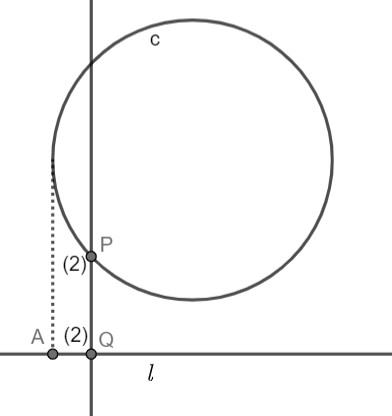
\includegraphics[width=0.4\textwidth]{kepek/kep16.png}
\end{figure}


Animation: $c$ and $l$ are fixed. $P$ is moving on $c$ with degree $2$, and $l$ is a line. Let the perpendicular projection of $P$ onto line $l$ be $Q$.

$Q$ has degree 2 also, so it passes through each point of $l$ 2 times with multiplicity. If we imagine the movement of $Q$, it halts at point $A$, and starts going backwards. $Q$ is at that position only once, but with multiplicity 2. That's because not only the distance of $A$ and $Q$ is 0, but the derivative of this distance is also 0. We say that the order of zero of the distance at this time is 2.

If the $i^{th}$ derivative of the distance is zero (for all $i=0,..., n-1$), but the $n^{th}$ is not, then the order of zero of the distance is $n$, and we say that the two points coincide with multiplicity $n$.

Similarly every statement has a natural multiplicity concept coming with it, usually the order of zero of some metric.

Let's go through some of them.

\begin{itemize}
    \item "$A=B$": The order of zero of the distance of $A$ and $B$
    \item "$e=f$": If $A$ and $B$ are the poles of lines $e$ and $f$ with respect to an arbitrary conic, then the multiplicity of "$A=B$"
    \item "$P$ lies on $l$": The order of zero of the distance of $P$ and $l$
    \item "$A, B, C$ are collinear": The order of zero of the area of triangle $ABC$
    \item "$e, f, g$ are concurrent": If $A$, $B$ and $C$ are the poles of lines $e$, $f$ and $g$ with respect to an arbitrary conic, then the multiplicity of "$A, B, C$ are collinear"
    \item "$\alpha=\beta$": The order of zero of $\alpha-\beta$
\end{itemize}

\begin{figure}[H]
    %\centering
    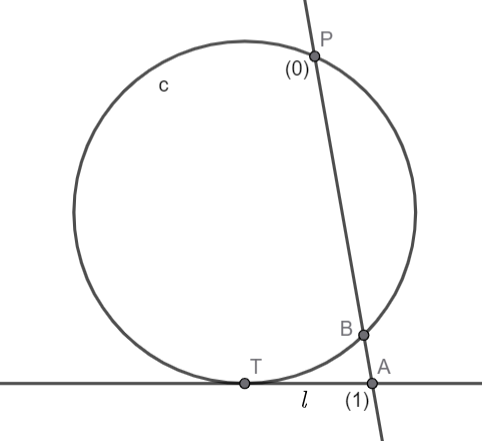
\includegraphics[width=0.5\textwidth]{kepek/kep17.png}
\end{figure}

$P$, $c$, $l$ are fixed, $A$ moves on $l$ with degree 1.

What is the multiplicity of "$A=B$" when $A=T$?

Calculate the degrees of $A$ and line $AB$.

Calculate the degree of $AB$ with the line through two points formula. The multiplicity of "$A=B$" should be the same as previously.

\subsection{Multiplicity of special cases}

We can use a special case multiple times. For example if the statement is that "$A, B, C$ are collinear", then if we show that they are collinear with multiplicity at least 2, it counts as two special cases. Of course they are collinear in every moment, but we can show that the order of zero of the area of triangle $ABC$ is at least 2.

For example when $A$ and $B$ coincide, the area  of $ABC$ must be 0. But if we take it further, and calculate the limes of line $AB$ it happens to pass through $C$. We know that the area of $ABC$ is $\frac{AB\cdot dist(AB, C)}{2}$, so it is the product of two at least order 1 zeros, so it is at least an order 2 zero.

Here we 'worked' for showing that $A=B$, then we 'worked' again to show that the limes of line $AB$ passes through $C$. So the rule of thumb is that whenever we 'work' for showing that the statement is true, we can raise the multiplicity of the special case by one.

\section{Square root points}\label{sqrt}

\subsection{Intersection of line and conic}

Let $\omega$ be a fixed conic, and $l$ be a polynomial moving line with degree $n$. Bad news: the two intersection points $P$ and $Q$ are not polynomial. Our current degree definition works only on polynomial points. Good news: there is a generalized degree definition, which works for $P$ and $Q$.

When calculating the coordinates of $P$ and $Q$, one has to solve a degree 2 polynomial, so square roots come in.

In fact, the coordinates of $P$ and $Q$ are from the set $$\{a+b\sqrt{H}\mid a,b \text{ are polynomials of time}\}$$
for some non-square polynomial of time $H$.

\subsection{Conjugate pairs}

Moreover $P$ and $Q$ are so-called conjugate pairs, this means the following:
$$P=(a+b\sqrt{H}:c+d\sqrt{H}:e+f\sqrt{H})$$
$$Q=(a-b\sqrt{H}:c-d\sqrt{H}:e-f\sqrt{H})$$

$\sqrt{H}$ cannot be defined over complex numbers as a continuous function, only $\pm \sqrt{H}$ as a two-valued function.

Analogously points $P$ and $Q$ cannot be distinguished, we can only talk about them as a pair.

\begin{definition}
    We say that $P$ and $Q$ form a square root point pair $(P,Q)$ if they are conjugate pairs.
\end{definition}

\begin{remark}
    A square root point/line form a pair with itself if and only if it is polynomial, because then the $\sqrt{H}$ part has zero coefficient in all three homogeneous coordinate.
\end{remark}



\subsection{Generalized degree}

We can define the generalized degree for square root object pairs, denoted by $\deg(P,Q)$. %citation here
The definition itself is quite ugly and unimportant, but knowing only its properties is enough for solving problems.
\begin{itemize}
    \item This degree can be half-integer, so for example degree $\frac{3}{2}$ points/lines can exist.
    \item This restricts to polynomial objects well, that is if we have a polynomial moving object $P$ with degree $n$, then the square root object pair $(P,P)$ has degree $n$ too.
    \item $\deg (P,Q)=\deg (Q,P)$
    \item The most important property comes in the next section, we will find out that the generalized degree can be calculated the same way as the polynomial degree.
\end{itemize}
  



\subsection{Constructing square root points}

If we apply a polynomial construction step to square root pairs $(P_1,Q_1), \ldots (P_k,Q_k)$ (that is applying the same construction to $P_1,\ldots P_n$ and $Q_1,\ldots Q_n$ respectively), the result will also be two square root objects, furthermore they will form a square root object pair. So one has to always keep in mind what the conjugate pair of an object is.

And a surprising fact, which should make the reader very happy is that the degree of the resulting pair should be calculated the same way as in the polynomial case. The only thing that you have to pay attention to is that whenever you count the number of times an event happens, count it with respect to $P_1,\ldots P_n$, and $Q_1,\ldots Q_n$, then take the average. Notice how the average is symmetric to the role of $P_1,\ldots P_n$ and $Q_1,\ldots Q_n$, and how this is necessary because we can't distinguish between the role of $P_i$ and $Q_i$. (Remark: We can correspond the $P$-s to each other, and the $Q$-s to each other, but we can't distinguish between the $P$-s and the $Q$-s. That's because in each $P_i$ we take $\sqrt{H}$ with a + sign, and in each $Q_i$ we take $\sqrt{H}$ with a - sign, and we can't distinguish between $+\sqrt{H}$ and $-\sqrt{H}$. But the 'choice' of $\pm\sqrt{H}$ happens only once, and not for every $i$ separately.)

Example:
\begin{theorem}
    Let $(P_1,P_2)$ and $(Q_1,Q_2)$ be two square root point pairs. Then the degree of square root line pair $(P_1Q_1, P_2Q_2)$ is

$$\deg (P_1Q_1, P_2Q_2)= \deg (P_1,P_2) + \deg (Q_1,Q_2) - \# ((P_1,P_2)=(Q_1,Q_2))$$

where $\# ((P_1,P_2)=(Q_1,Q_2))=\sum_{t\in \cc\pp^1} \frac{\operatorname{mul}_t(P_1=Q_1)+\operatorname{mul}_t(P_2=Q_2)}{2}$.
\end{theorem}
\begin{remark}
    Square root point pairs don't move in a complex differentiable way as polynomials did. That is because $\sqrt{H}$ is not complex differentiable when $H(t)=0$. So this means that the order of zero of $a+b\sqrt{H}$ can be half-integer too. Luckily this only happens when $P(t)=Q(t)$ in a square root pair $(P,Q)$, that is they are the same at a time $t$. And when this happens both $a+b\sqrt{H}$ and $a-b\sqrt{H}$ have integer+0.5 multiplicity, so their sum is an integer as usual. The problem is that until now we could assume that if an event happens, it happens with at least multilplicity 1. But now it can happen with multiplicity 0.5 in these cases. But again, this is only a problem if $P=Q$, so always have an eye on this condition while working with square root points.
\end{remark}
The next lemma tells us what the degree of the intersection of a line a fixed conic is.
\begin{lemma}
    Let $\omega$ be a fixed conic, and $l$ be a polynomial moving line. The two intersection points of $\omega$ and $l$ are $P$ and $Q$. Then $(P,Q)$ form a degree $\deg l$ square root point pair.
\end{lemma}
\begin{proof}
    $P$ and $Q$ are the intersection of a fixed conic a moving line, and we can calculate their coordinates. It turns out that they have square roots in their coordinates, furthermore they are conjugate pairs. Since Mászó-theorem also holds for square root points,
    $$\frac{\deg(P,Q)+\deg(QP)}{2}=\deg (PQ,QP)=\deg l$$
    $(P,Q)$ and $(Q,P)$ have the same degree, so their degrees are equal to their average. Therefore $\deg (P,Q)=\deg l$ 
\end{proof}

\subsection{Degree of statements}
We can apply a polynomial statement to square root object pairs $(P_1,Q_1), \ldots (P_k,Q_k)$ (that is applying the statement to $P_1,\ldots P_n$ and $Q_1,\ldots Q_n$ respectively), and get a square root statement pair $(S_1,S_2)$. $S_1$ and $S_2$ are conjugate to each other.
The degree of a square root statement pair $(S_1,S_2)$ is defined as
$$\deg(S_1,S_2)=\sum_{t\in \cc\pp^1} \frac{\operatorname{mul}_t(S_1)+\operatorname{mul}_t(S_2)}{2}$$
The degree of a square root statement pair $(S_1,S_2)$ can be calculated the same way as in the polynomial case.

A degree $n$ square root statement pair $(S_1,S_2)$ is either true $n$ times on average, or $"S_1$ or $S_2"$ is always true. This means that if we find $n+0.5$ or more special cases, we proved that in every moment either $S_1$ or $S_2$ is true. If we prove only one of $S_1$ and $S_2$, it counts as 0.5 case on average, however if we prove both $S_1$ and $S_2$, it counts as 1 case.

This result is not quite that useful at first, since we can't guarantee that both $S_1$ and $S_2$ are true, only that in every moment either $S_1$ or $S_2$ is true. But in most cases the latter implies the former:

\begin{theorem}
    Let $(S_1,S_2)$ be a non-polynomial square root statement pair. If in every moment $S_1$ or $S_2$ is always true, then both $S_1$ and $S_2$ are always true.
\end{theorem}

If an object pair $(P_1,P_2)$ is non-polynomial, then a statement pair $(S_1,S_2)$ constructed form it is non-polynomial too. (or $S_1=S_2$ in which case the theorem holds too) 

The most common way to show that we a have non-polynomial square root statement pair is to find a degree of an object which is integer+0.5. Obviously polynomial objects don't have such degrees.

\subsection{Angle bisector}
\begin{theorem}
    Let $\alpha$ be a polynomial varying angle. Then $\left(\frac{\alpha}{2},\frac{\alpha}{2}+90^{\circ}\right)$ is a square root angle pair with degree $\frac{\deg\alpha}{2}$.
\end{theorem}
\begin{proof}
    Let $\tan\alpha=\frac{p}{q}$, where $p$ and $q$ are degree $\deg\alpha$ polynomials of time with no common root.

    The equation $2x=\alpha$ modulo $180^{\circ}$ has two solutions, $\frac{\alpha}{2}$ and $\frac{\alpha}{2}+90^{\circ}$. We can use the tangent half angle formula to get
    $$\tan \left(\frac{\alpha}{2}(+90^{\circ})\right)=\frac{-1\pm\sqrt{1+\tan^2\alpha}}{\tan\alpha}=\frac{-q\pm\sqrt{q^2+p^2}}{p}$$
    So they indeed form a square root conjugate pair.
    Since $2\deg \beta=\deg (2\beta)$ for a polynomial varying angle $\beta$, this works just the same in the square root case, therefore
    $$2\deg\left(\frac{\alpha}{2},\frac{\alpha}{2}+90^{\circ}\right)=\deg (\alpha, \alpha)=\deg \alpha$$
\end{proof}

\begin{example}
    Let $l$ be a degree 1 line rotating around the origin. Then the inner and outer angle bisectors of $l$ and the x-axis are square root line pairs with degree $0.5$.
    \begin{proof}
        The angle between $l$ and the x-axis has degree 1. Then the half-angles corresponding to the inner and outer angle bisectors form a square root pair of degree 0.5. Then the angle bisectors themselves form a square root line pair of degree 0.5. 
    \end{proof}
\end{example}



\subsection{Example problem}

\begin{exercise}[IMOSL 2022 G7]
    Two triangles $ABC, A’B’C’$ have the same orthocenter $H$ and the same circumcircle with center $O$. Letting $PQR$ be the triangle formed by $AA’, BB’, CC’$, prove that the circumcenter of $PQR$ lies on $OH$.
\end{exercise}

\begin{proof}
    \begin{figure}[H]
    \centering
    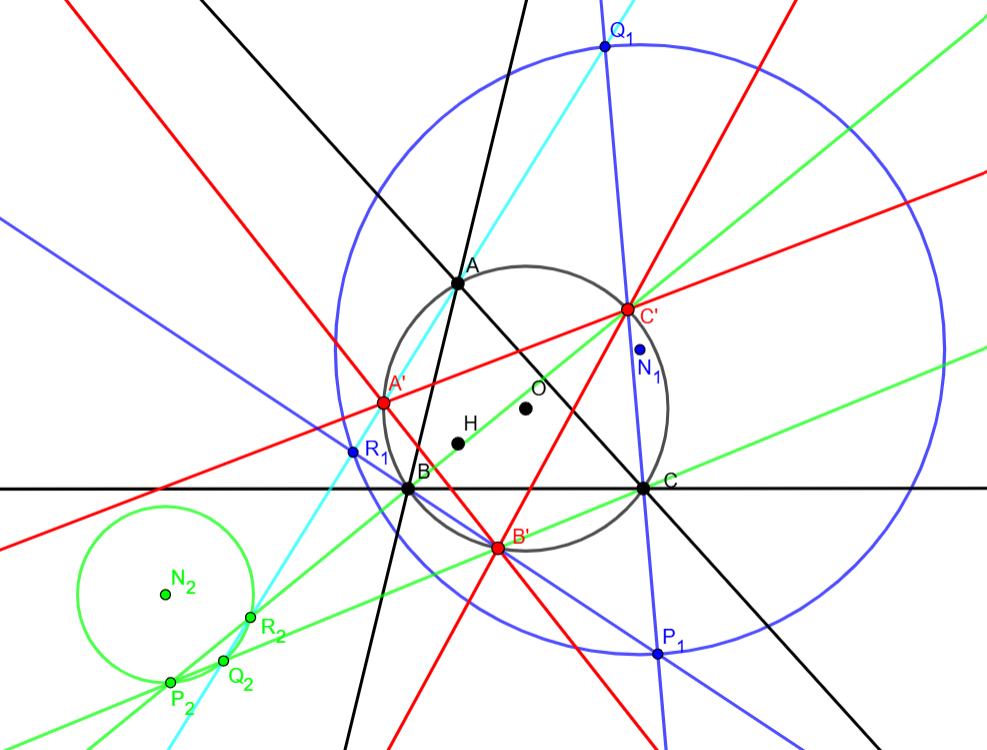
\includegraphics[width=0.9\textwidth]{kepek/kep18.png}
    \end{figure}

Let us fix \(A\), \(B\), \(C\), \(O\), \(H\), \(G\), \((ABC)\) and let us vary \(A_1\) along \((ABC)\) where \(\deg A' = 2\). Since \(\triangle ABC\) and \(\triangle A'B'C'\) have the same orthocenter and circumcircle, hence they have the same centroid \(G\).
Since
\[
\frac{A'G}{GM} = \frac{2}{1},
\]hence \(\deg M = \deg A' = 2\).
Hence
\[
\deg OM = \deg O + \deg M - \#(O = M) = 0 + 2 - 0 = 2.
\]Hence \(\deg \infty_{OM} = 2\).
Since \(B'C' \perp OM\), hence \(\deg \infty_{B'C'} = 2\) as well. Then
$$\deg M\infty_{B'C'}=\deg M+\deg \infty_{B'C'}-\#(M=\infty_{B'C'})=2+2-2=2$$
One of the coincidences of $M$ and $\infty_{B'C'}$ happen when $A=\alpha_i$, because here $M=\alpha_i$ too (applying scaling to $\alpha_i$ doesn't change it). Furthermore $\infty_{OM}=\alpha_i$, thus $\infty_{B'C'}=\alpha_i$. The other coincidence is when $A=\alpha_{-i}$ for the same reason.

A degree 2 polynomial line intersects the fixed $(ABC)$ in a degree 2 square root point pair $(B',C')$. The fixed $B$ forms a degree 0 square root pair with itself: $(B,B)$. So the square root line pair connecting the square root point pairs $(B',C')$ and $(B,B)$ is $(B'B,C'B)$. Applying the square root Mászó-theorem we get
$$\deg (B'B,C'B)=\frac{\deg (B',C')+\deg (B,B)}{2}=\frac{2+0}{2}=1$$
Similarly we get that lines $B'C$ and $C'C$ also form a square root line pair, and its degree is 1.
Line $AA'$ is polynomial and by Mászó-theorem, its degree is 1.
Now $P_1$, $Q_1$, $R_1$ are points formulated by lines $AA', BB', CC'$ (blue lines). And logical symmetrically let $P_2$, $Q_2$, $R_2$ be their conjugate pair, that is the points formulated by lines $AA'$, $BC'$, $CB'$ (green lines).
Since $P_1=BB'\cap CC'$ and $P_2=BC'\cap CB'$ we can apply the square root version of the formula for the intersection of two lines to get the degree of $(P_1,P_2)$:
$$\deg (P_1,P_2)=\deg (BB',BC')+\deg (CC',CB')-\#((BB',BC')=(CC',CB'))=1+1-0.5=1.5$$
where $\#((BB',BC')=(CC',CB'))=\sum_{t\in \cc\pp^1} \frac{\operatorname{mul}_t(BB'=CC')+\operatorname{mul}_t(BC'=CB')}{2}$

Let's count the average multiplicity of the coincidence:
Since $B$ and $C$ are fixed points, $BB'=CC'$ or $CC'=CB'$ can only happen when ($B'=C$ and $C'=B$) or ($B'=B$ and $C'=C$). This can only happen when $A'=A$. In this case one of the pairs $(BB',CC')$ and $(BC',CB')$ is $(BC,BC)$ and the other is the tangents to $(ABC)$ at $B$ and $C$. (we don't know which is which, but it is unnecessary since the average multiplicity is symmetric). So one of ($\operatorname{mul}_t(BB'=CC'), \operatorname{mul}_t(BC'=CB')$) is 1 and the other is 0, so on average the two lines coincide 0.5 times.

Next, calculate the degree of $(Q_1,Q_2)$. $AA'$ is polynomial, so $(AA',AA')$ form a square root line pair. $(Q_1,Q_2)$ is the intersection of $(AA',AA')$ and $(CB',CC')$.
$$\deg (Q_1,Q_2)=\deg (AA',AA')+\deg (CB',CC')-\#((AA',AA')=(CB',CC'))=1+1-0.5=1.5$$
Line pairs $(AA',AA')$ and $(CB',CC')$ can coincide only if $A'=C$. In this case $(AA',AA')=(AC,AC)$ and $(CB',CC')=(AB,AC)$. Therefore one of the coincidences happen, and the other doesn't, so the number of average coincidences is 0.5.

By the same calculation $\deg (R_1,R_2)=1.5$.

In the polynomial case, the formula for the circumcircle is the following:
$$\deg (PQR)= 2(\deg P+\deg Q+\deg R)-\#(\text{"any two points are the same" or "any point is one of the circle points"}$$
$$\text{or "any 2 points are on the ideal line" or "all 3 points are collinear on a line with slope $i$ or $-i$"})$$
This has a square root version too, where we take pairs instead, and the number of events that make the degree drop is taken with the average multiplicity.

Foreshadowing the result,
$$\deg ((P_1Q_1R_1),(P_2,Q_2,R_2))=2(1.5+1.5+1.5)-6.5=2.5$$

Now let's count the number of events, where we can reduce the degree. It should be 6.5 in total.

\begin{itemize}
    \item (0.5) $A'=A$ One of the following happen: $"BC'=CB'"$, $"BB'=CC'$. So one of the following will happen: $"Q_1=R_1"$, $"Q_2=R_2"$. However, the other event won't happen, so we can reduce the degree by average of 0.5.
    \item (0.5) $A'=B$ Similarly, two lines will coincide in one of the triangles, making two points coincide in one of the triangles. We can reduce by 0.5.
    \item (0.5) $A'=C$ Symmetric to previous.
    \item (1) $A'=\alpha_i$ We've already seen that $\infty_{B'C'}=\alpha_i$ and we know that $B'C'$ always goes through the midpoint of $HH'$, where $H'$ is the mirror image of $H$ w.r.t. $B'C'$, making $H'\in (A'B'C')$. This midpoint however is a finite (complex) point on the line $HA=H\alpha_i$. Therefore line $B'C'$ is also $H\alpha_i$. Thus one of $B'$, $C'$ is $\alpha_i$ and the other is $H'$ (some random complex, finite point). Let's say $B'=\alpha_i$ (it could be that $C'=\alpha_i$, but the same argument works then, this is just to ease the notation). $BB'$ and $AA'$ both have slope $i$, and they are not the same line, so their intersection $P_1$ is $\alpha_i$. In the same way $CB'$ and $AA'$ both have slope $i$, so $P_2=\alpha_i$ too. So $P_1$ and $P_2$ coincide with $\alpha_i$ an average of 1 time.
    \item (1) $A'=\alpha_{-i}$ Same argument works.
    \item (2) One of $AA',BB',CC'$ and $AA',BC',CB'$ are concurrent at a finite point, and no two lines are the same from the three. There are two cases (it is clear in geogebra) when this happens. Let's suppose it happens with $AA',BB',CC'$. Then $P_1, Q_1, R_1$ are all at this concurrency point (no two lines are the same). This counts as multiplicity 2 conincidence, so we can reduce the degree by average of $\frac{0+2}{2}=1$. This happens twice, so in total we reduce by 2.
    \item (1) $A'$ is the mirror image of $A$ w.r.t. $OH$. Then one of $AA',BB',CC'$ and $AA',BC',CB'$ are all perpendicular to $OH$, and no two are the same line, so all 3 intersections $(P_1, P_2, P_3)$ are the same ideal point. This again counts as a multiplicity 2 coincidence, so we can reduce the degree by an average of 1.
    
\end{itemize}

So $\deg ((P_1Q_1R_1),(P_2,Q_2,R_2))=2.5$ (or less, but the solution works nevertheless). These circles are never the ideal line counted twice, so their midpoints $(N_1,N_2)$ form a degree 2.5 square root point pair.

$(OH, OH)$ is a degree 0 square root line pair.

The statement that $"(N_1,N_2)$ lies on $(OH, OH)"$ has degree $2.5+0=2.5$. Therefore in total we need $3$ cases to show that $N_1$ OR $N_2$ lies on $OH$. Since we had some degree 1.5 point pairs, these square root pairs must be irreducible. From this it follows that $N_1$ AND $N_2$ lies on $OH$.

\begin{itemize}
    \item (0.5) $A'=C$ One of the triangles $P_1Q_1R_1$ and $P_2Q_2R_2$ coincide with $ABC$, so their circumcircle are the same too. So in average this counts as 0.5 case.
    \item (0.5) $A'=B$ Symmetric to the previous.
    \item (0.5)  $A'$ is the mirror image of $A$ w.r.t. $OH$. We've seen that one of the triangles $P_1Q_1R_1$ and $P_2Q_2R_2$ is a single ideal point, but the other is a proper triangle, which is symmetric to $OH$. This means that its circumcircle is also on $OH$.
    \item (0.5) $A'=A$ One of the triangles is formulated by the tangents to $(ABC)$ in $A$, $B$ and $C$. This is elementary geo...
    \item (1) One of $AA',BB',CC'$ and $AA',BC',CB'$ are concurrent at a finite point, and no two lines are the same from the three. There are two cases (it is clear in geogebra) when this happens. Then the circumcircle of the degenerate triangle in the concurrency point is again that point, and this should be on $OH$, this elementary again. Two such cases lead to 1 case in average.
\end{itemize}
    
    
\end{proof}

\section{Choosing the best animation}
(unfinished section)
\begin{exercise}[APMO 2024 1]
    Let $ABC$ be an acute triangle. Let $D$ be a point on side $AB$ and $E$ be a point on side $AC$ such that lines $BC$ and $DE$ are parallel. Let $X$ be an interior point of $BCED$. Suppose rays $DX$ and $EX$ meet side $BC$ at points $P$ and $Q$, respectively, such that both $P$ and $Q$ lie between $B$ and $C$. Suppose that the circumcircles of triangles $BQX$ and $CPX$ intersect at a point $Y \neq X$. Prove that the points $A, X$, and $Y$ are collinear.
\end{exercise}

\begin{exercise}[APMO 2024 5]
    Line $\ell$ intersects sides $BC$ and $AD$ of cyclic quadrilateral $ABCD$ in its interior points $R$ and $S$, respectively, and intersects ray $DC$ beyond point $C$ at $Q$, and ray $BA$ beyond point $A$ at $P$. Circumcircles of the triangles $QCR$ and $QDS$ intersect at $N \neq Q$, while circumcircles of the triangles $PAS$ and $PBR$ intersect at $M\neq P$. Let lines $MP$ and $NQ$ meet at point $X$, lines $AB$ and $CD$ meet at point $K$ and lines $BC$ and $AD$ meet at point $L$. Prove that point $X$ lies on line $KL$.
\end{exercise}

\begin{exercise}
    Let $ABCD$ be a convex quadrilateral. Let $M$ and $N$ be the midpoints of the sides $AB$ and $CD$ respectively. The line $MN$ intersects the diagonals $AC$ and $BD$ at $P$ and $Q$ respectively. Prove that the circles $BMQ$ and $CNP$ intersect each other on the line $BC$.
\end{exercise}

\begin{exercise}
    Let $P$, $Q$ be isogonal conjugate points wrt. $\Delta ABC$. Point $X$ is the orthogonal projection of $Q$ on $BC$. The circle with diameter $PA$ intersects $(ABC)$ at $K\ne A$. $AQ$ intersects $(ABC)$ at $T\ne A$. Prove that the points $K$, $X$, $T$ are collinear.
\end{exercise}

\section{Incircle animation advanced techniques}
(unfinished section)
\begin{exercise}
    Let $ABC$ be a triangle with circumcenter $O$ and incenter $I$. The $A$-mixtilinear incircle has center $K$ and tangency points $T$, $E$ and $F$ on $(ABC)$, $AC$, $AB$ resp. $AI$ intersects $BC$ in $S$, $TI$ intersects $BC$ in $N$. Circle $(AEF)$ intersects $AN$ in $G\ne A$, and $(ABG)$ intersects $AI$ in $Q\ne A$. Prove that $B$, $F$, $Q$, $S$ are concyclic.
\end{exercise}

\section{Help! I can't imagine circle points!}
(unfinished section)

We often require to see clearly what happens when some points of the figure become one of the circle points. Often we have to calculate some multiplicity, or the limit of a moving object at a certain time when it is not defined. But how to calculate anything when the circle points are complex points at infinity? We can't even imagine them. But luckily, there is a technique with which we can draw a situation around the circle points, we will first understand it, and then we look at some examples.



\section{Length and area}
(unfinished section)
\subsection{Length of segments}

\begin{definition}
     The complex length-square $(AB)^2$ of segment $AB$ is defined to be $(a_x-b_x)^2+(a_y-b_y)^2$, this is a complex number.
\end{definition}

\begin{theorem}
    Let $A$ and $B$ be polynomial moving points. Then the complex length-square $(AB)^2$ of segment $AB$ is a polynomial quantity with degree
    $$\deg (AB)^2=2\deg A+2\deg B-$$
    $$-\sum_{t\in\cc\pp^1}\min\Big(\ord(A,B,\alpha_i\text{ collinear})+\ord(A,B,\alpha_{-i}\text{ collinear}),$$
    $$2\ord(A\in \text{ideal line})+2\ord(B\in \text{ideal line})\Big)$$
\end{theorem}
\begin{remark}
    The multiplicity $\ord(A,B,C\text{ collinear})$ is the order of zero of the area of the triangle $ABC$ according to any chart containing $A$, $B$ and $C$.
    
    The multiplicity $\ord(P\in l)$ is the order of zero of the distance of $P$ from $l$ according to any chart containing $P$.
\end{remark}
\begin{remark}
    If either $A$ or $B$ is at one of the circle points (say $A$), then we can reduce the degree by at least one, since then $"A\in \text{ideal line}"$ is true, and $"A,B,\alpha_i\text{ collinear}"$ is also true (or with $\alpha{-i}$).

    If both $A$ and $B$ are ideal points, then we can reduce by at least 2, since then both $"A,B,\alpha_i\text{ collinear}"$ and $"A,B,\alpha_{-i}\text{ collinear}"$ are true, and also $2\ord(A\in \text{ideal line})+2\ord(B\in \text{ideal line})\ge 4$, so we are good on that side by far.
\end{remark}
\begin{proof}
$A=(a_0:a_1:a_2)$ and $B=(b_0:b_1:b_2)$.




With euclidean coordinates
$$|AB|^2=\left(\frac{a_0}{a_2}-\frac{b_0}{b_2}\right)^2+\left(\frac{a_1}{a_2}-\frac{b_1}{b_2}\right)^2=\frac{(a_0b_2-b_0a_2)^2+(a_1b_2-b_1a_2)^2}{(a_2b_2)^2}$$
So 
with homogeneous coordinates in $\cc\pp^1$ this is
$$|AB|^2=\big((a_0b_2-b_0a_2)^2+(a_1b_2-b_1a_2)^2:(a_2b_2)^2\big)$$
Now cancel the common factor in these homogeneous coordinates:

These are degree $2\deg A+2\deg B$ polynomials, and we have to subtract $\sum_{t\in\cc\pp^1}\ord\Big(|AB|^2=(0,0)\Big)$ from this to get the degree of $|AB|^2$
$$\ord\Big(|AB|^2=(0,0)\Big)\overset{\text{by def}}{=}\min\Big(\ord\big((a_0b_2-b_0a_2)^2+(a_1b_2-b_1a_2)^2\big), \ord\big((a_2b_2)^2\big)\Big)=$$
$$\min\Big(\ord\big([-i(a_0b_2-b_0a_2)+(a_1b_2-b_1a_2)][i(a_0b_2-b_0a_2)+(a_1b_2-b_1a_2)]\big), \ord\big((a_2b_2)^2\big)\Big)=$$
$$\min\Big(\ord\big(-i(a_0b_2-b_0a_2)+(a_1b_2-b_1a_2)\big)+\ord\big(i(a_0b_2-b_0a_2)+(a_1b_2-b_1a_2)\big), 2\ord(a_2)+2\ord(b_2)\Big)=$$
$$\min\left(\ord\left(\det
\begin{bmatrix}
a_0 & a_1 & a_2 \\
b_0 & b_1 & b_2 \\
1 & i & 0
\end{bmatrix}
\right)+\ord\left(\det
\begin{bmatrix}
a_0 & a_1 & a_2 \\
b_0 & b_1 & b_2 \\
1 & -i & 0
\end{bmatrix}
\right),
2\ord((a_0,a_1,a_2)\cdot(0,0,1))+2\ord((b_0,b_1,b_2)\cdot(0,0,1))\right)=$$
$$\overset{\text{see below}}{=}\min\Big(\ord(A,B,\alpha_i\text{ collinear})+\ord(A,B,\alpha_{-i}\text{ collinear}), 2\ord(A\in \text{ideal line})+2\ord(B\in \text{ideal line})\Big)$$

By the determinant definition of collinearity, $\ord(A,B,\alpha_i\text{ collinear})=\ord\left(\det
\begin{bmatrix}
a_0 & a_1 & a_2 \\
b_0 & b_1 & b_2 \\
1 & i & 0
\end{bmatrix}
\right)$

Also, $\ord(A\in \text{ideal line})=\ord\big((a_0,a_1,a_2)\cdot(0,0,1)\big)=\ord(a_2)$, where this is a dot product.
\end{proof}

\section{Random problems with solutions}

\begin{exercise}[2026 USAJMO P3]
    Let $ABC$ be an acute scalene triangle with no angle equal to $60^{\circ}$. Let $\omega$ be the circumcircle of $ABC$. Let $\triangle_B$ be the equilateral triangle with three vertices on $\omega$, one of which is $B$. Let $\ell_B$ be the line through the two vertices of $\triangle_B$ other than $B$. Let $\triangle_C$ and $\ell_C$ be defined analogously. Let $Y$ to be the intersection of $AC$ and $\ell_B$, and let $Z$ be the intersection of $AB$ and $\ell_C$.

Suppose that the circumcircle of $AYZ$ intersects $\omega$ at $P\neq A$, $BC$ intersects $YZ$ at $D$, and $PA$ intersects $YZ$ at $E$. Prove that $PE=PD$.
\end{exercise}
\begin{proof}
    figure here

    Fix $B$, $C$, $\omega$, and with this $\ell_B$ and $\ell_C$. Move $A$ on $\omega$ with degree 2.

    Then $BA$, $CA$ have degree 1 by Mászó-theorem. Their intersections with fixed lines $\ell_C$ and $\ell_B$ are $Z$ and $Y$, which thus have degree 1.

    Line $ZY$ have degree $1+1-0=2$.

    In fact since $\deg ZY=2$, it touches a fixed conic. We can point at 6 cases, when $ZY$ is one of the sides of $\Delta_B$ or $\Delta_C$, therefore it touches the circle concentric to $\omega$ with half radius.

    Circle $(AYZ)$ has degree $2(1+1+2)-6=2$, where the 6 cases where we can reduce are
    when $A$ is on either $\ell_B$ or $\ell_C$ causing $A=Y$ or $A=Z$ (4 cases) and when $A=\alpha_i$ or $A=\alpha_{-i}$.

    Circle $\omega$ and $(AYZ)$ have two intersection points $A$ and $P$. Since $A$ is polynomial, $P$ is so, and the sum of their degrees is $\deg A+\deg P=2(0+2)-0=4$. $A$ has degree 2, so $P$ has degree 2.

    Line $PA$ has degree 2 by Mászó-theorem.

    The intersection of $YZ$ and $PA$ is $E$, which then has degree $2+2-0=4$.

    The intersection of $YZ$ and $BC$ is $D$, which then has degree $2+0-0=2$.

    The complex length-square of $PD$ has degree $2(2+2)-2=6$, and the 2 cases of reducing happen when $P=\alpha_i$ and $P=\alpha{-i}$.

    The complex length-square of $PE$ has degree $2(2+4)-6=6$, and the 6 cases of reducing happen when $YZ$ has slope $i$ and $-i$, both with multiplicity 3. When $YZ$ has slope $i$, it goes through the center $O$ of $\omega$, since $YZ$ is always tangent to a circle with center $O$. Let us determine the position of every other object:

    $(AYZ)$ is the conic thorugh $A$, $Y$, $Z$, $\alpha_i$, $\alpha_{-i}$, in this case $Y,Z,\alpha_i$ are collinear, so $(AYZ)$ is the union of lines $O-Y-Z-\alpha_i$ and $A\alpha_{-i}$.

    If we draw the situation through a projective transformation sending the circle points to finite points, we get the following (note that line $O\alpha_i$ is tangent to $\omega$):

    figure here

    Therefore the 4 intersection points $A$, $P$, $\alpha_i$ and $\alpha_{-i}$ of $\omega$ and $(AYZ)$ are $A=\text{random finite complex point}$, $\alpha_i$ counted twice and $\alpha_{-i}$, therefore $P=\alpha_i$. Then $E=PA\cap YZ$ is the intersection of $A\alpha_i$ and $O\alpha_i$, which is also $\alpha_i$, so $E=\alpha_i$.

    But the story does not end here. Now imagine that the time moves a little bit.
    
    figure here
    
    Then $YZ$ moves a little while being tangent to $\omega$, and $P$ moves a little on $\omega$. Then the distance of $P$ and $E$ has order of zero 2. Also $\alpha_i$ and line $PE$ has order of zero 1, and since the area of triangle $PE\alpha_i$ is half the product of these two distances, it has order of zero 3. Also both $P$ and $E$ lie on the ideal line, so $2\ord(A\in \text{ideal line})+2\ord(B\in \text{ideal line})\ge 4$, so $\min\Big(\ord(A,B,\alpha_i\text{ collinear})+\ord(A,B,\alpha_{-i}\text{ collinear}),$$
    $$2\ord(A\in \text{ideal line})+2\ord(B\in \text{ideal line})\Big)=3$, and thus we can reduce by 3.

    So all in all, both length-square of $PD$ and length-square of $PE$ has degree 6 (these are polynomial quantities, or moving points on $\cc\pp^1$ in other words). The statement is that these are equal, this has degree $6+6=12$, so we need 13 cases.

    (4 cases) $P=A$ happens 2 times, when $AB=AC$, then $|PD|^2=|PE|^2$ with multiplicity at least two, because then by symmetry both $D$ and $E$ are ideal points, therefore both $|PD|=\infty$ and $|PE|=\infty$, so $|PD|^2=\infty$ and $|PE|^2=\infty$ with multiplicity two, which means that on $\cc\pp^1$, their distance from the infinite point has order of zero 2, and thus $|PD|^2$ and $|PE|^2$ has order of zero 2 from each other.

    (1) $Y=\infty$ ... I'm lazy, sorry :)
\end{proof}



%%%%%%%%%%%%%%%%%%%%%%%%%%%%%%%%%%%%%%%%%%%%%%%%%%

\bibliographystyle{plain}
\bibliography{forrasok}

Supported by the EKÖP-25 university research scholarship program of the ministry for culture and innovation from the source of the national research, development and innovation fund.


\end{document}
